\documentclass[11pt,compress,professionalfonts]{beamer}
\usepackage[]{graphicx}
\usepackage[]{color}
\usetheme{metropolis}

\usepackage{mathspec}
\setsansfont{Avenir Next}[BoldFont={* Demi Bold}]
%[BoldItalicFont={* Demi Bold Italic},
%ItalicFont={* Italic},
%BoldFont={* Demi Bold},
%UprightFont={* Regular}]
\setmonofont[Scale = MatchLowercase,Mapping=tex-ansi]{Inconsolata}
\setmathfont(Digits,Latin,Greek){Avenir Next}
\definecolor{pton}{HTML}{EE7F2D}

\setbeamercolor{frametitle}{fg=white, bg=pton}
\metroset{progressbar=none,numbering=none}
%\setbeamercolor{progress bar in head/foot}{fg=pton,bg=darkgray}

\usepackage{ctable}
\usepackage{hyperref}
\usepackage{dcolumn}
\usepackage{booktabs}
\newcommand{\ita}{\begin{itemize}}
\newcommand{\itm}{\item[]}
\newcommand{\itz}{\end{itemize}}

\IfFileExists{upquote.sty}{\usepackage{upquote}}{}

\graphicspath{{pics/}}

\title{Computer-assisted content analysis}
%\subtitle{It begins\ldots}
\author{Will Lowe ~~Princeton University\\James Lo ~~ University of Southern California}
\institute{IQMR 2016 Syracuse}

\begin{document}

\maketitle


%
%How to model categorical $\theta$ without specifying a dictionary and without having a training set?
%
%Example questions:
%
%Simple case: What proportion of weblogs strongly dislike, dislike, are indifferent to, like or strongly like Kerry as a candidate?
%
%Harder case: How does the balance of topics in a corpus change over time?
%

%\slide{Topic Models 1}

%\centerline{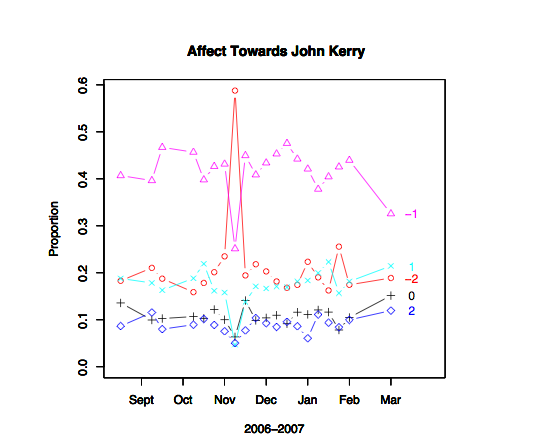
\includegraphics[scale=.8]{kerry-blogs}}
%


\begin{frame}[t,fragile]\frametitle{Menu}

Session 1: Classical Content Analysis

Session 2:
\ita


\itm Classification for Known Categories: Supervised Methods
\itm Evaluation
\itm Content Analysis Research Design
\itz

Session 3: Topic and Scaling Models


\end{frame}
\begin{frame}[t,fragile]\frametitle{Text as Data}

\centerline{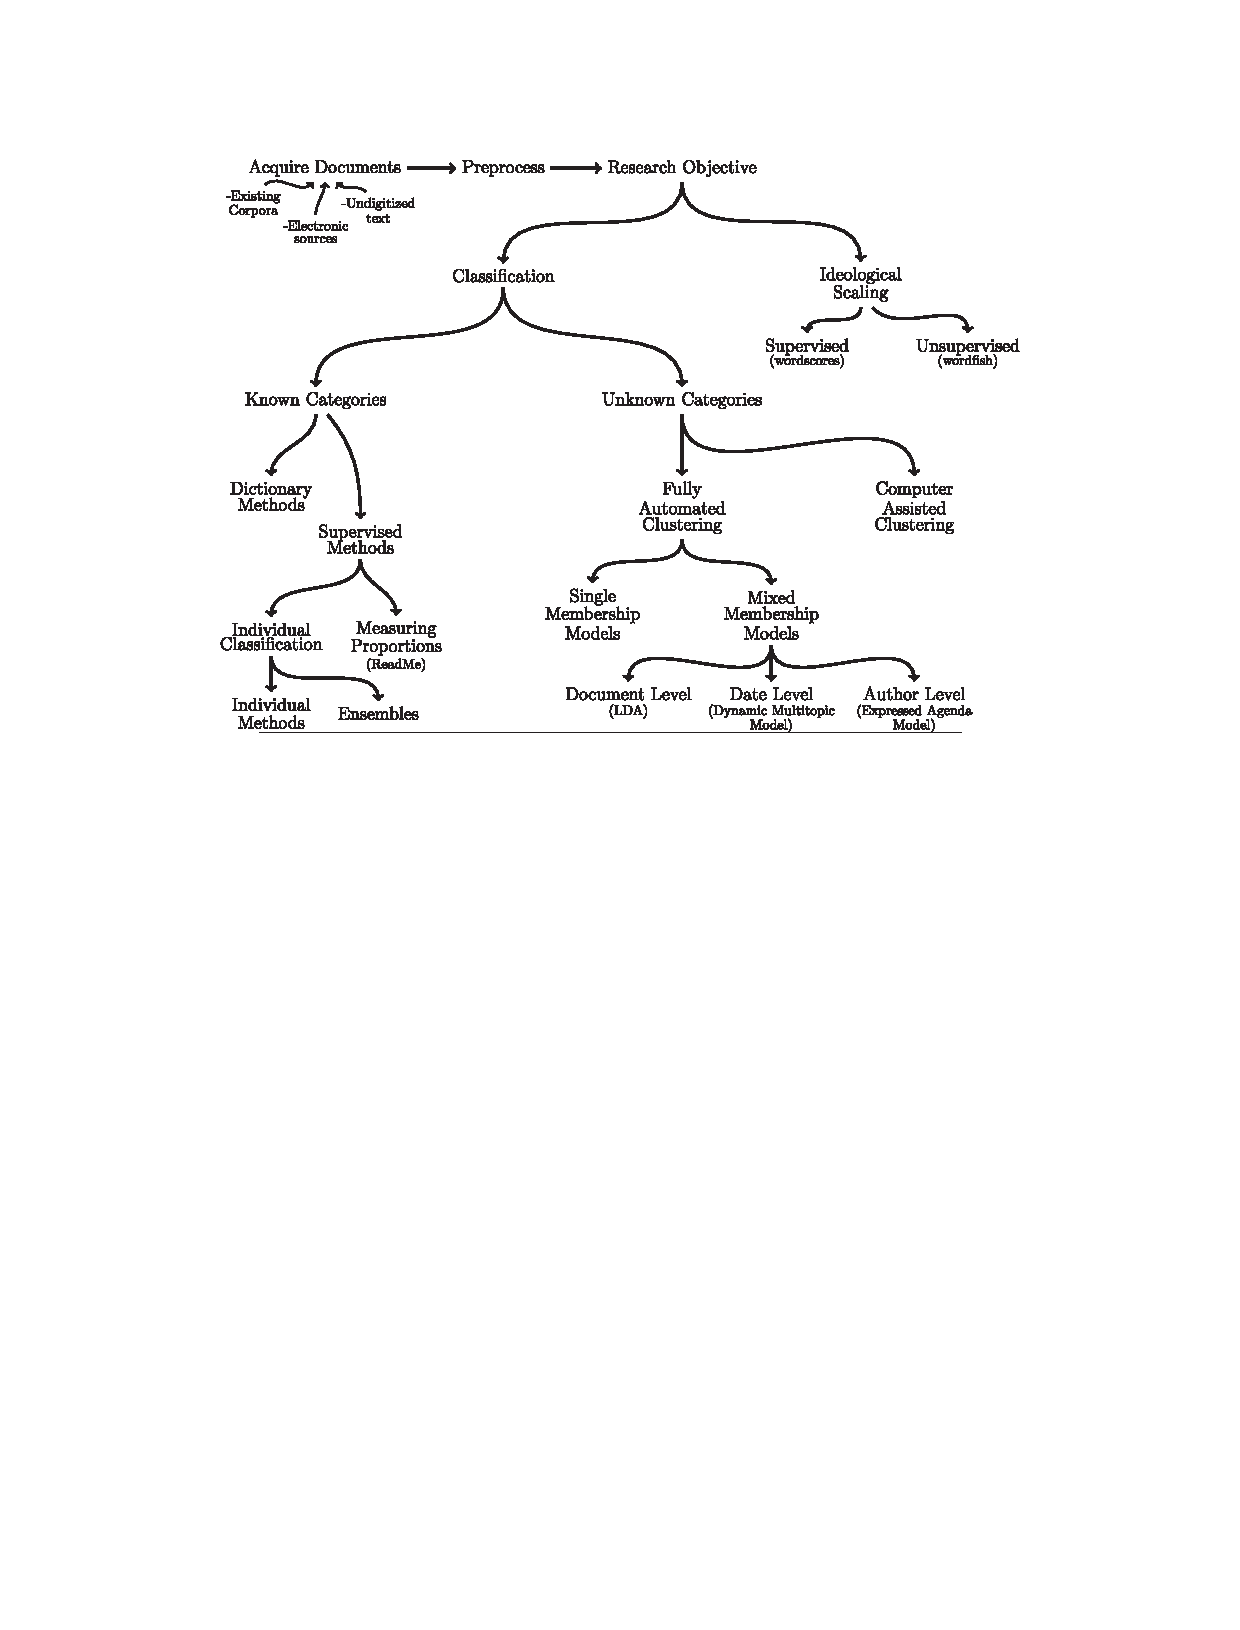
\includegraphics[scale=1]{grimmerovreview.pdf}}
\centerline{\footnotesize Source: Grimmer and Stewart (2013)}




%%%%%%%%%%%%%%%%
%%%%%%%%%%%%%%%%

\end{frame}
\begin{frame}[t,fragile]\frametitle{Classification Approaches when Categories are Known}

{\bf Examples:}

Are campaign advertisements positive or negative?

What  policy areas do newspaper editorials cover?

Are international statements belligerent or peaceful?

Do court letters represent liberal or conservative positions?

What language is this article written in?

Is this email spam?

\end{frame}
\begin{frame}[t,fragile]\frametitle{Classification Approaches when Categories are Known}

Earlier today, we talked how to do this using a dictionary approach.

An alternative are supervised machine learning methods.

The idea:

\begin{enumerate}

\item coders categorize a set of documents by hand
\item the algorithm ``learns" how to sort the documents in categories
\item  characteristics of training set are used  to assign new documents to categories.
\end{enumerate}


\end{frame}
\begin{frame}[t,fragile]\frametitle{Classification Approaches when Categories are Known}

Assume that each document has a \textit{single} topic Z

Let $\theta_k$ be the \textit{probability} that Z=k for each document

Assume that (some) topic labels are observed



%We can \textit{choose} a style of model\\
%~\\

%\centerline{\includegraphics[scale=.7]{classification-plate}~~~~~~~~~
%\includegraphics[scale=.7]{classification-plate2}}

%\centerline{Discriminative Style ~~~~~~~~~~~~~~~~ Generative Style}

\end{frame}
\begin{frame}[t,fragile]\frametitle{Classification Approaches}

\centerline{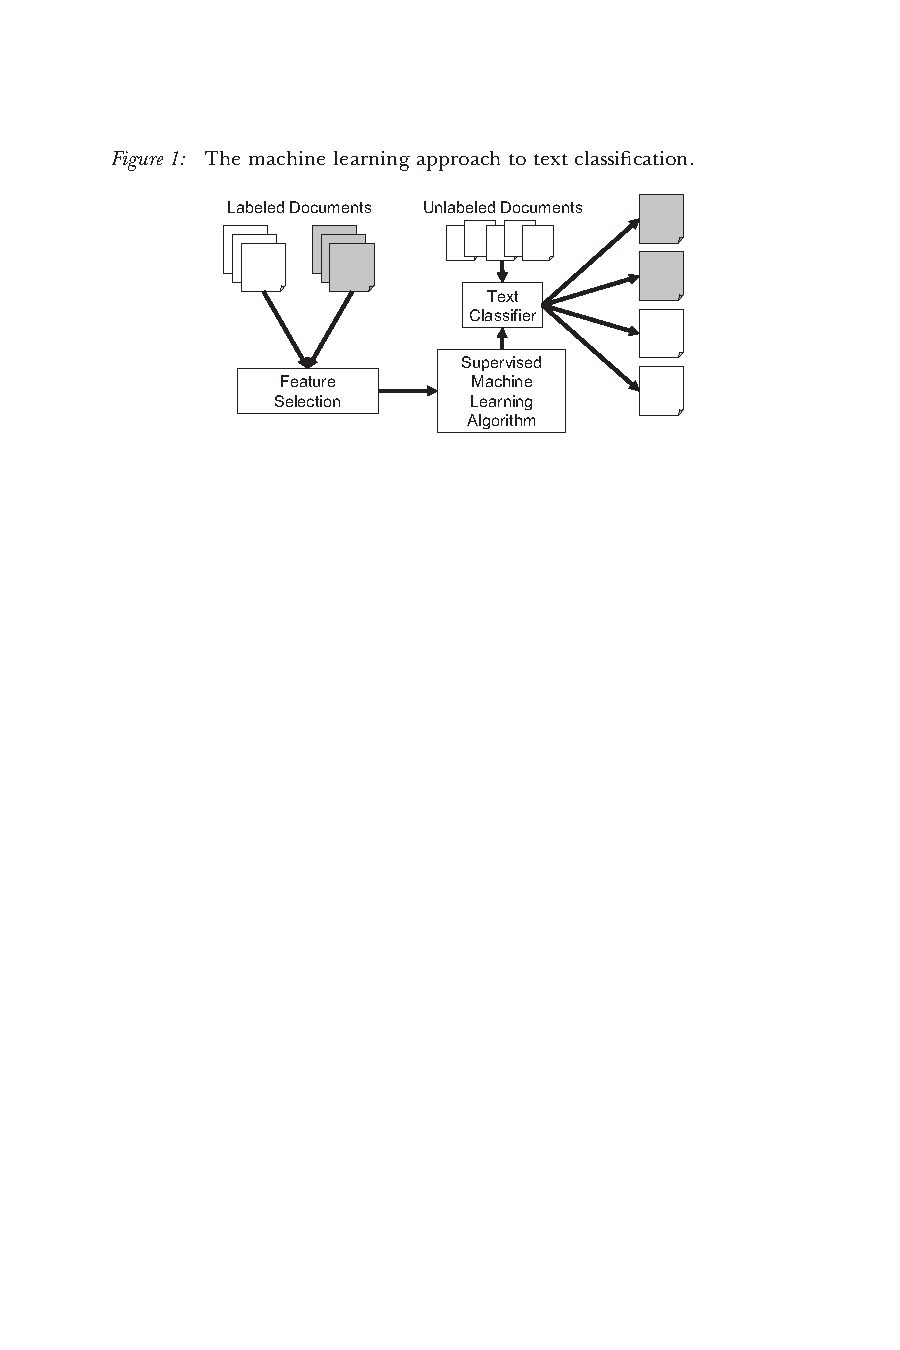
\includegraphics[scale=1]{evans1.pdf}}

\end{frame}
\begin{frame}[t,fragile]\frametitle{Output}

Desirable classification outcome:

\begin{center}
\begin{tabular}{lcc}
& $P(Z=`\text{Domestic Policy}'\mid \text D)$ & $P(Z=`\text{Foreign Policy}' \mid \text D)$ \\ \toprule
$D_1$ & 0.75 & 0.25 \\
$D_2$ & 0.82 & 0.18 \\
\ldots & \ldots & \ldots\\
$D_{N-1}$ & 0.02 & 0.98 \\
$D_N$ & 0.45 & 0.55\\ \bottomrule
\end{tabular}
\end{center}

\end{frame}
\begin{frame}[t,fragile]\frametitle{The Basic Steps}

\begin{enumerate}

\item Construct a training set

(a) create a coding scheme\\
(b) select documents (ideally randomly sampled)

\item Apply the supervised learning method to learn features of a training set and infer labels

\item Validate and classify remaining documents

\end{enumerate}

\end{frame}
\begin{frame}[t,fragile]\frametitle{Caveats}

Much of machine learning, computational linguistics, and AI deals with classification problems
\ita
\itm We only touch on the issues here\ldots
\itz
%Individual classifiers: naive Bayes, support vector machines, neural networks, $\ldots$

Ensembles: combine different individual classifiers to produce one that is superior to any of the individual ones.


\end{frame}
\begin{frame}[t,fragile]\frametitle{Example of Naive Bayes Classifier: Amicus Curiae Briefs}

Background:
\ita
\itm Amicus Curiae (friend of the court) briefs are submitted to an appellate court
\itm They usually present a legal argument for or against one of the parties to a case
\itm Amicus Curiae can be submitted by any group that feels that it has a stake in the case
\itz

\end{frame}
\begin{frame}[t,fragile]\frametitle{Affirmative action}

Evans et al. use cases about the constitutionality of `affirmative action' programs at university level.

%\ita
%\itm Regents of the University of California vs. Bakke (1978)
%\itm Grutter vs Bollinger, Lehman, Shields, and the Regents of the University of Michigan (2003)
%\itm Gratz and Hamacher vs Bollinger, Lehman, Shields and the Regents of the University of Michigan (2003)
%\itz
The arguments are as much \textsl{political} (state vs federal rights, social welfare, constitutional interpretation) as they are \textsl{legal}

\end{frame}
\begin{frame}[t,fragile]\frametitle{Affirmative Action}

This work uses document classification to answer two questions
\ita
\itm To what extent can the conservative/liberal \textsl{direction} of an AC brief be predicted on the basis of its words?
\itm What can we learn about \textsl{language} of each side of the case?
\itz

\end{frame}
\begin{frame}[t,fragile]\frametitle{Naive Bayes}

\textsl{Naive Bayes} is a relatively old ($\sim$1975)  classification method

Suppose one had to guess  whether document $j$ is liberal (Z=L) or conservative (Z=C) based on its word profile $W_j$.

Probability can be derived by applying Bayes theorem:

\begin{align*}
P(Z=L \mid W_j) &~=~ \frac{P(W_j \mid Z=L)~P(Z=L)}{P(W_j)}
\end{align*}

\end{frame}
\begin{frame}[t,fragile]\frametitle{Naive Bayes}

\begin{align*}
P(Z=L \mid W_j) &~\propto~ P(W_j \mid Z=L)~P(Z=L)
\end{align*}

We can drop $P(W_j)$ since it is constant across categories.

Given a representative training set, estimating $P(Z=L)$ is easy:

\begin{align*}
\hat{P}(Z=L)&~=~ \frac{\text{\# training docs that are liberal}}
{\text{\# of training docs}}
\end{align*}

\end{frame}
\begin{frame}[t,fragile]\frametitle{Naive Bayes}

Estimating the probability that a word profile $W_j$ occurs given that the document is liberal $P(W_j\mid Z=L)$ is more challenging, because any one word profile is likely to occur only once.

Solution: words are assumed to be generated \textit{independently} given the category Z (the `naive' and wrong assumption).
\begin{align*}
P(W_j \mid Z=L) &~=~ \prod_i P(W_i \mid Z=L)\\
&~=~ \prod_i P(W_i \mid \theta_L) ~~~~~~\text{realised as Multinomial or Binomial}
\end{align*}
\newpage

\end{frame}
\begin{frame}[t,fragile]\frametitle{Naive Bayes}

With this assumption, we can estimate the probability of observing a word $i$  given that the document is liberal: proportion of word $i$ in liberal training set.

The classifier then  chooses the class Z (Liberal or Conservative) with the highest aggregate probability.

Note that every new word adds a bit of information that re-adjusts the conditional probabilities.

\newpage


\end{frame}
\begin{frame}[t,fragile]\frametitle{Naive Bayes}



Note that with two classes (here: liberal and conservative)  this has a rather neat interpretation:
\begin{align*}
\frac{P(Z=\text{`Liberal'} \mid W_j)}
{P(Z=\text{`Conservative'} \mid W_j)} = \\
~~~~~~~~~\prod_i \frac{P(W_i \mid Z=\textsl{`Liberal'})}
{P(W_i \mid Z=\textsl{`Conservative'})}\times \frac{P(Z=\textsl{`Liberal'})}{~P(Z=\textsl{`Conservative'})}
\end{align*}
Logging this probability ratio, every new word \textsl{adds} a bit of information that pushes the ratio above or below 0
%
%\slide{Naive Bayes}
%
%Example: Naive Bayes with only word class `discriminat*'.
%\begin{align*}
%P(W=\text{`discriminat*'} \mid Z=\text{`Liberal'}) & = {70}/{17368} \approx 0.004\\
%P(W=\text{`discriminat*'} \mid Z=\text{`Conservative'}) & = {26}/{20002} \approx 0.001
%\end{align*}
%Assume that liberal and conservative supporting briefs are equally likely (not true, but\ldots)
%\begin{align*}
%\frac{P(Z=\text{`Liberal'})}{P(Z=\text{`Conservative'})} & = 1
%\end{align*}
%
%Last step:  calculate posterior classification  probabilities for a new document (based on occurrence of this word).
%
%\slide{Naive Bayes}
%
%A Priori we estimate that this ratio is 1
%
%Now we look an Amicus brief from `King County Bar Association' containing 3667 words%(File 6019\_al18-utf8.txt)
%
%This contains 4 matches to disciminat*.
%
%\slide{Naive Bayes}
%
%A priori, the probabilities are\ldots
%
%Probability that we observe the word  discriminat* 4 out of 3667 times if the document is liberal: .00007
%
%Probability that we observe the word  discriminat* 4 out of 3667 times if the document is conservative: .18311
%
%Now, we just need to calculate the posterior probabilities using the logged probability ratio\ldots
%
%\newpage
%
%\slide{Naive Bayes}
%
%Conclusion: Seeing 4 instances of discriminat* gives the posterior classification probabilities
%\ita
%\itm $\theta_\text{liberal}$ = 0.996
%\itm $\theta_\text{conservative}$ =  1-0.996=0.004
%\itz
%
%This is quite confident
%\ita
%\itm \ldots but other words will be less loaded or push the other way
%\itz
%
%
%


\end{frame}
\begin{frame}[t,fragile]\frametitle{Evaluating Classifiers:\\Accuracy, Precision and Recall}

How can we evaluate how good a supervised classifier works?

Use the confusion matrix (training set versus machine)


\end{frame}
\begin{frame}[t,fragile]\frametitle{Evaluating Classifiers:\\Accuracy, Precision and Recall}

\begin{center}
\scalebox{0.7}{
\begin{tabular}{llcc}
\toprule
&&\multicolumn{2}{c}{Machine}\\
\cline{3-4}
&& Liberal & Conservative \\
\midrule
Training Data & Liberal & 40&10\\
& Conservative &40&60\\
\bottomrule
\end{tabular}}
\end{center}

\vspace*{0.5cm}

Accuracy = (40+60)/150 = .66

Precision ($Z_{machine}$=Liberal) = 40/(40+40) = 0.5

Precision ($Z_{machine}$=Cons) = 60/(10+60) = 0.86

Recall ($Z_{training}$=Liberal) = 40/(40+10) = 0.80

Recall ($Z_{training}$=Cons) = 60/(40+60) = 0.60


\end{frame}
\begin{frame}[t,fragile]\frametitle{Evaluation}

Use evaluation to improve classifier. Things you can do:

\ita
\itm refine coding scheme for human coding
\itm ensure representative training set
\itm use ensemble of classifiers

\itz

\end{frame}
\begin{frame}[t,fragile]\frametitle{Distinctive Words}

Detecting different rhetorical styles of liberal and conservative groups:

``Liberal groups use language emphasizing the impact of affirmative action polices, while conservative words indicate concern over legal-constitutional limits on administrative procedure'' (Evans et al. 2007, p. 1029)

\newpage

\centerline{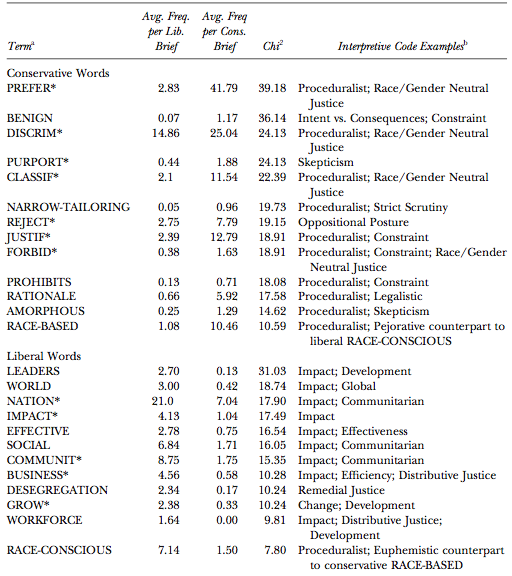
\includegraphics[scale=1]{words-evans}}
%
%\slide{Refresher on $\chi^2$}
%
%A $\chi^2$ \textsl{statistic} is computed as
%\begin{align*}
%\frac{(\text{observed} - \text{expected})^2}{\text{expected}}
%\end{align*}
%In large samples it has a $\chi^2$ \textsl{distribution}.
%
%For measuring how useful a term would be in a classifier we are more interested in magnitude
%
%
%\slide{Refresher on $\chi^2$}
%
%\begin{center}
%\begin{tabular}{llll}
%            & purport* & not purport*   & \\ \midrule
%petitioners & 43       & 166101       & 166144 \\
%respondents & 34       & 673552       & 673586 \\ \midrule
%            & 77       & 839653       & 839730
%\end{tabular}
%\end{center}
%
%If purport* words occurred at the \textsl{same} rate then their expected proportion would be
%\[
%\frac{77}{839730}
%\]
%
%
%If \textit{not} we would estimate the rates as
%\begin{align*}
%\text{conservatives:} && \frac{43}{166144}\\
%\text{liberals:} && \frac{34}{673586}
%\end{align*}
%
%
%The $\chi^2$ asks whether the observed counts are probable under the assumption that words occur at the \textsl{same} rate. Conservatives use purport* words at more than 5 times the rate of liberals.\\
%\begin{align*}
%\frac{43~/~166144}{34~/~673586} & = 5.127
%\end{align*}
%
%\newpage
%Evans et al. 2007: "Many conservatives doubt that diversity is "narrowly tailored" to achieve a compelling state interest as "purported," or that it actually delivers many of its "alleged" benefits." (p.1030)
%
%
%\newpage
%\centerline{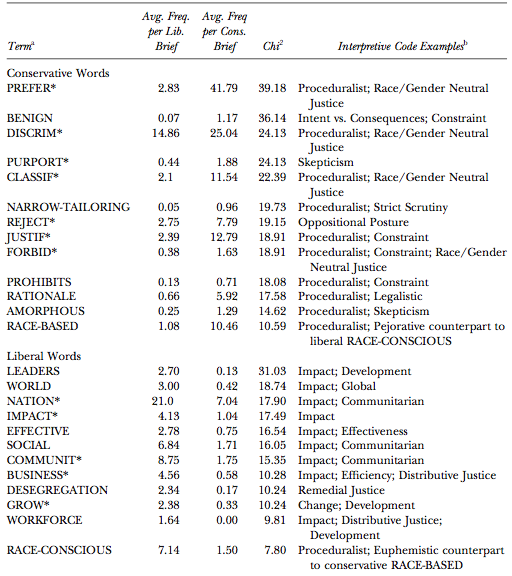
\includegraphics[scale=.9]{words-evans}}

\end{frame}
\begin{frame}[t,fragile]\frametitle{Compare and Contrast}

Bara et al. (2007) abortion debate with a thematic dictionary
\begin{center}
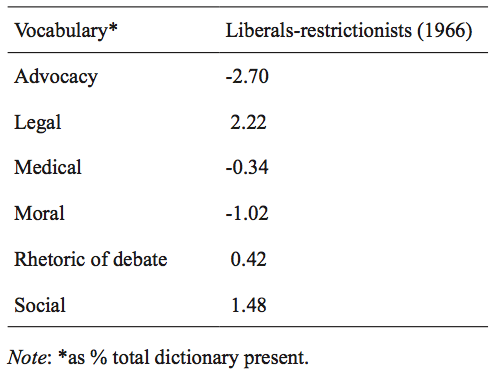
\includegraphics[scale=1]{bara-diffs}
\end{center}

\end{frame}
\begin{frame}[t,fragile]\frametitle{Vocabulary Usage}

We can use known Z to characterize vocabulary usage directly, if we're careful\ldots

Monroe et al. (2008) compare different measures of `partisan vocabulary' in abortion debates
\ita
\itm Simple frequencies will be misleading
\itm They settle for Laplace regularized odds-ratios
\itz


\end{frame}
\begin{frame}[t,fragile]\frametitle{Vocabulary Usage}

\centerline{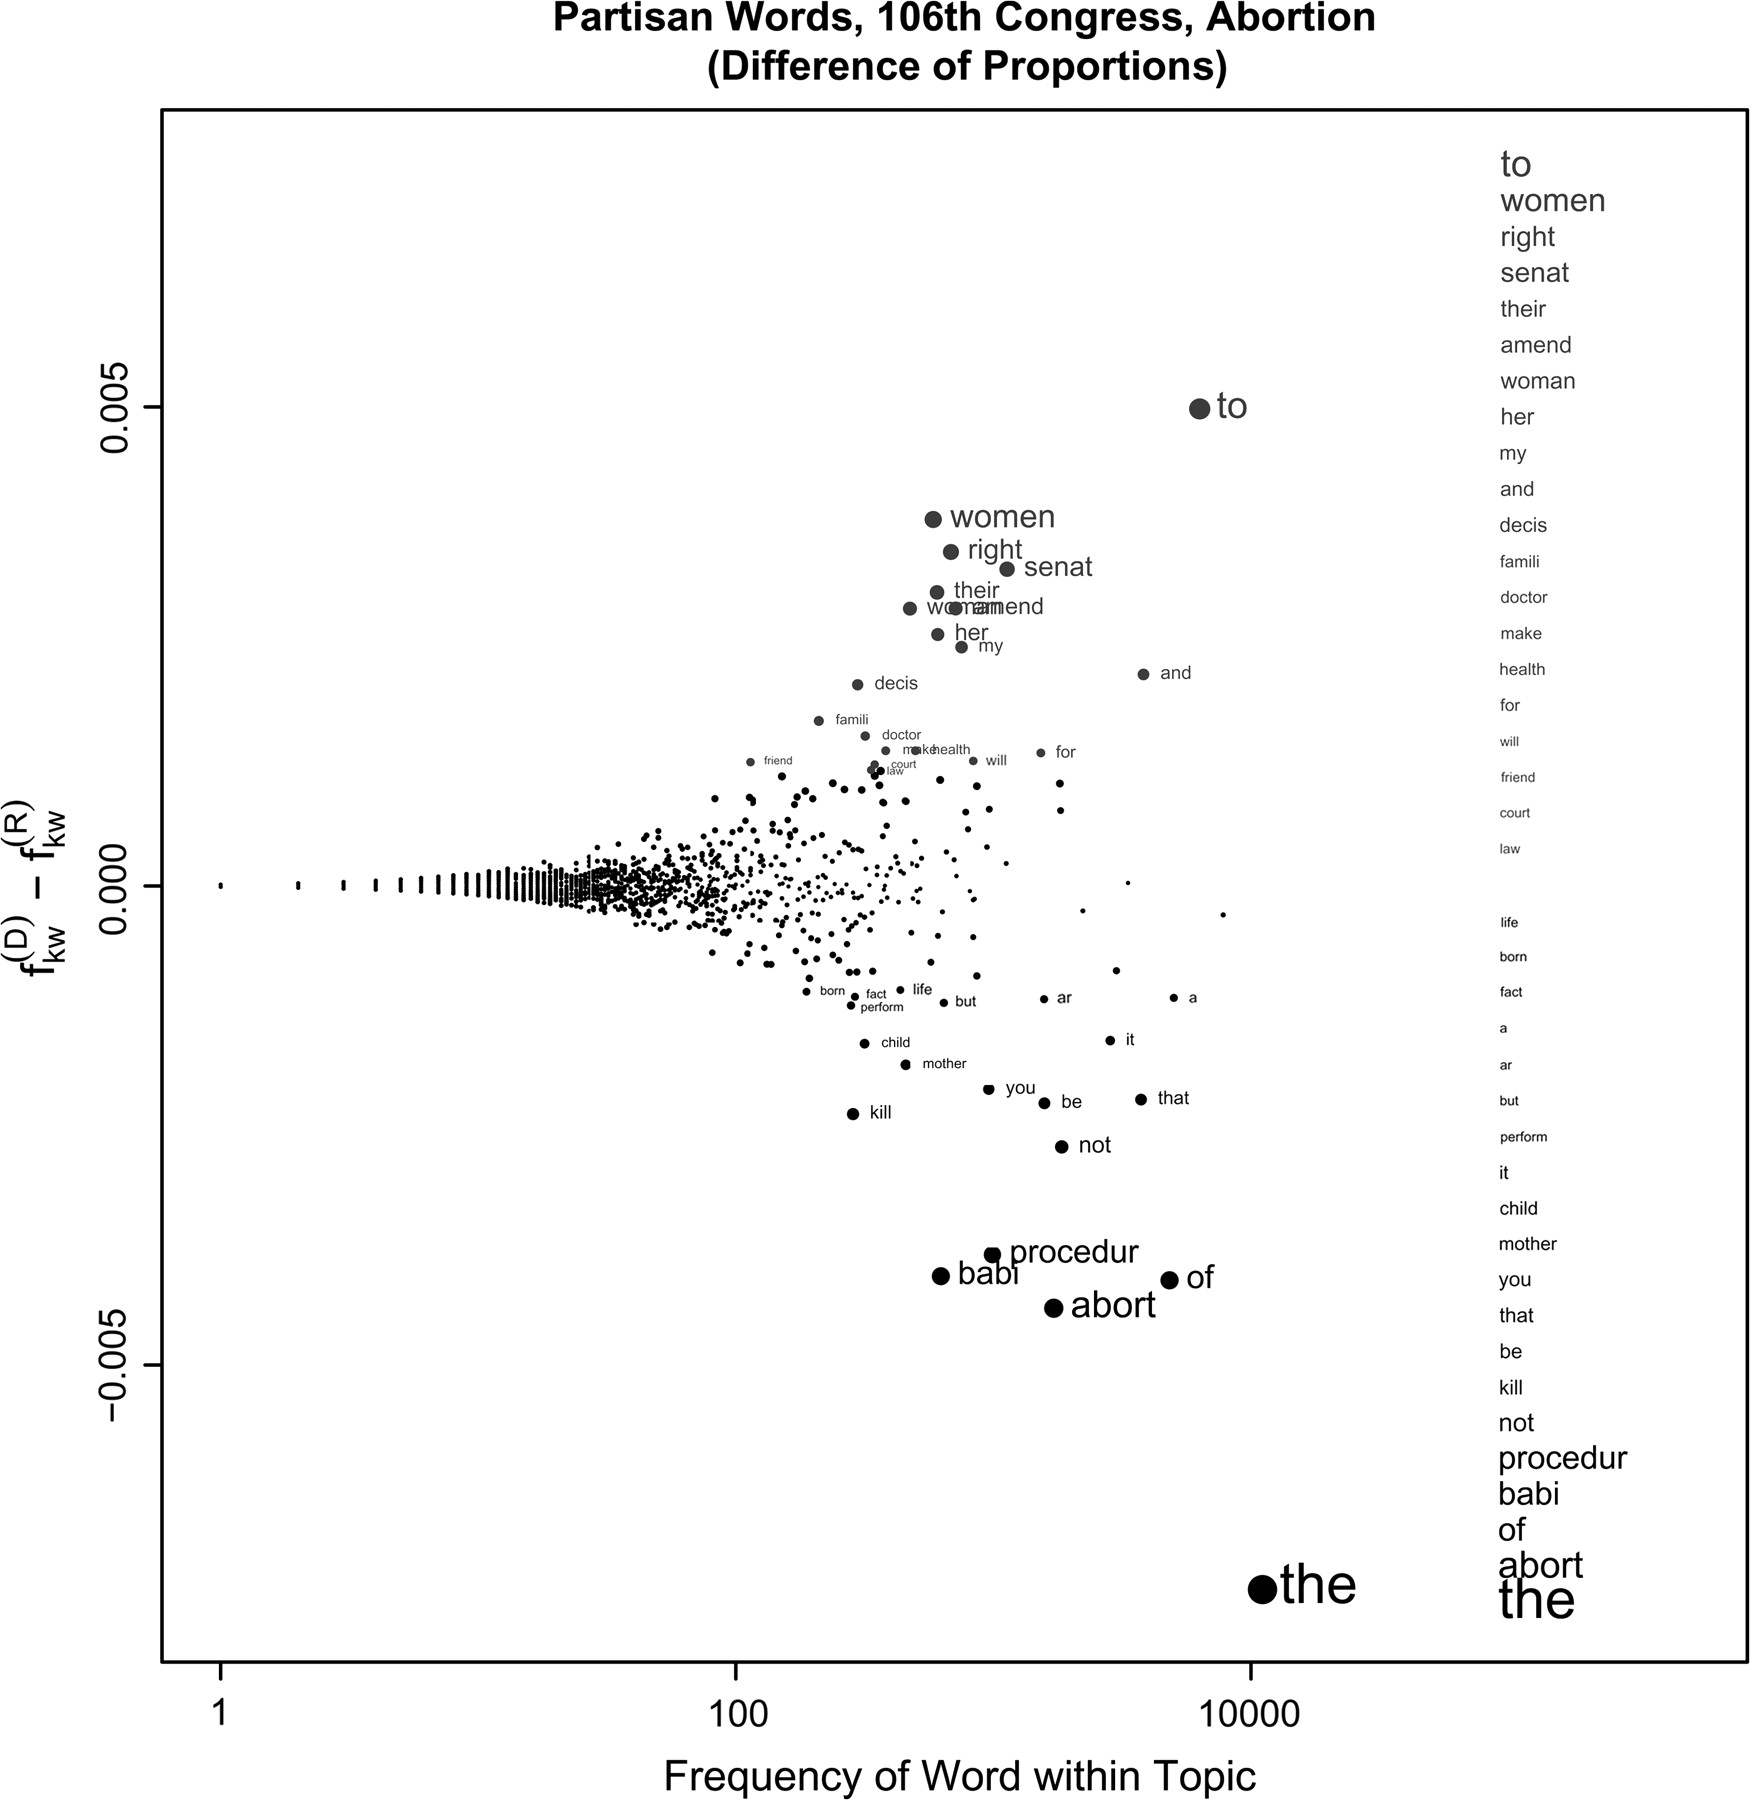
\includegraphics[scale=.2]{fightin0}}

{\footnotesize Difference of proportions: could result in lack of overall semantic validity due to the overemphasis on high-frequency words, unclear which words matter (Monroe et al. 2009).}

\end{frame}
\begin{frame}[t,fragile]\frametitle{Vocabulary Usage}

\centerline{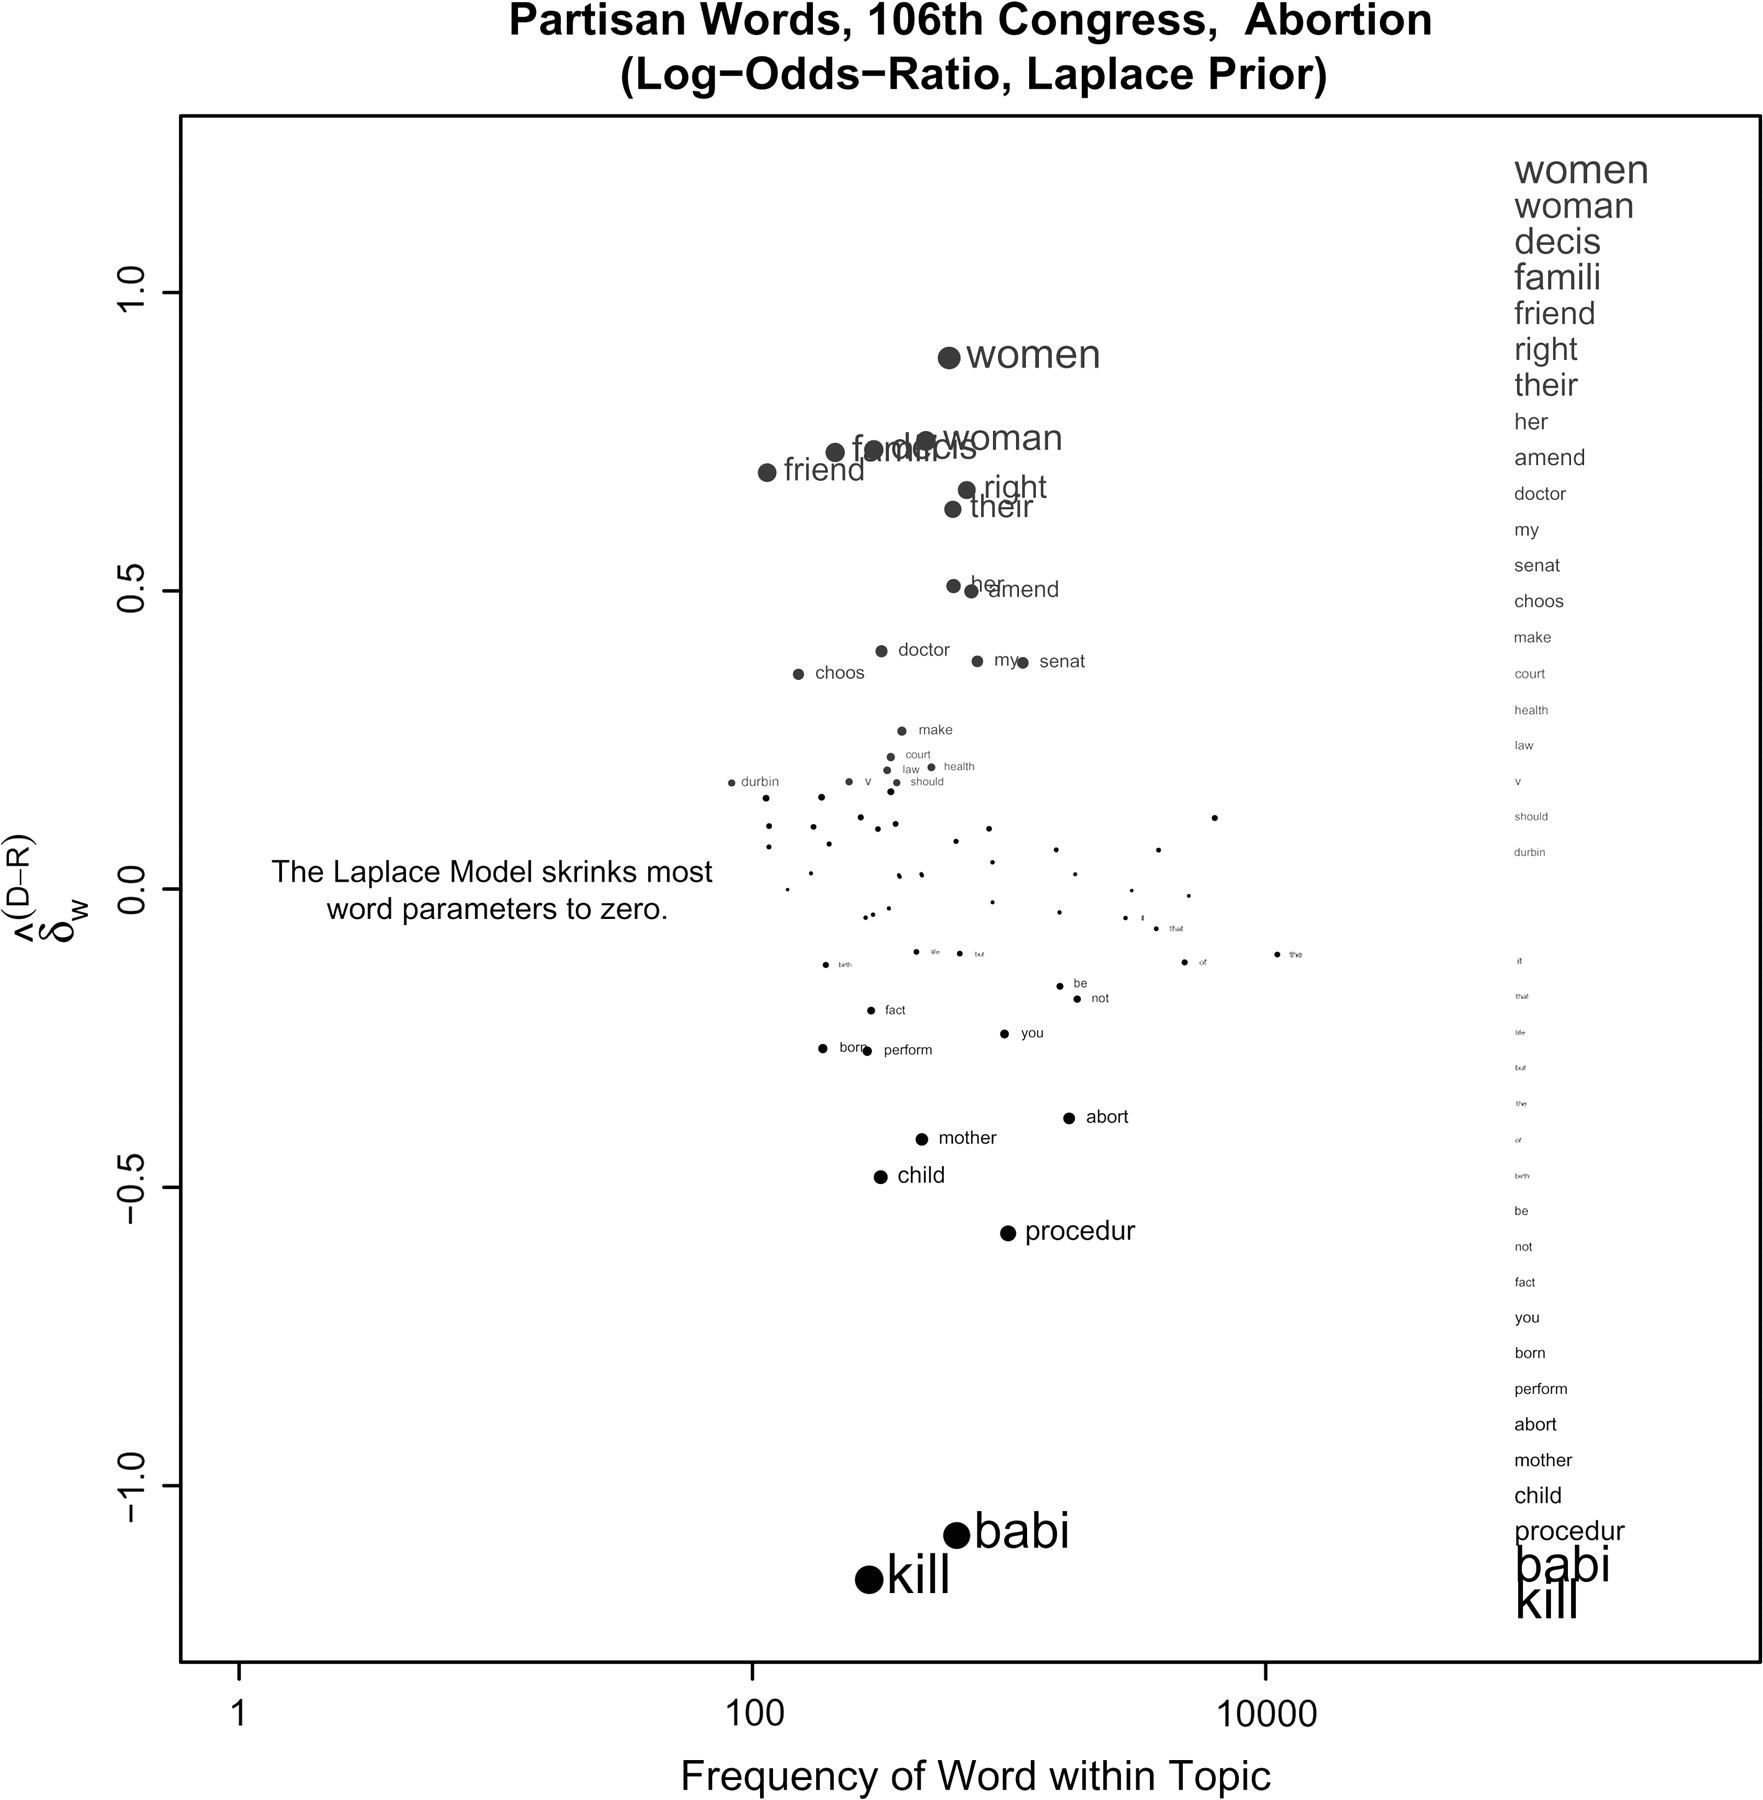
\includegraphics[scale=.2]{fightin1}}

{\footnotesize An additional prior means that words whose partisanship is not clear will receive partisan contrasts that are exactly zero. Identifying important words is now easier (Monroe et al. 2009).}

\end{frame}
\begin{frame}[t,fragile]\frametitle{Lexical Instability}

\centerline{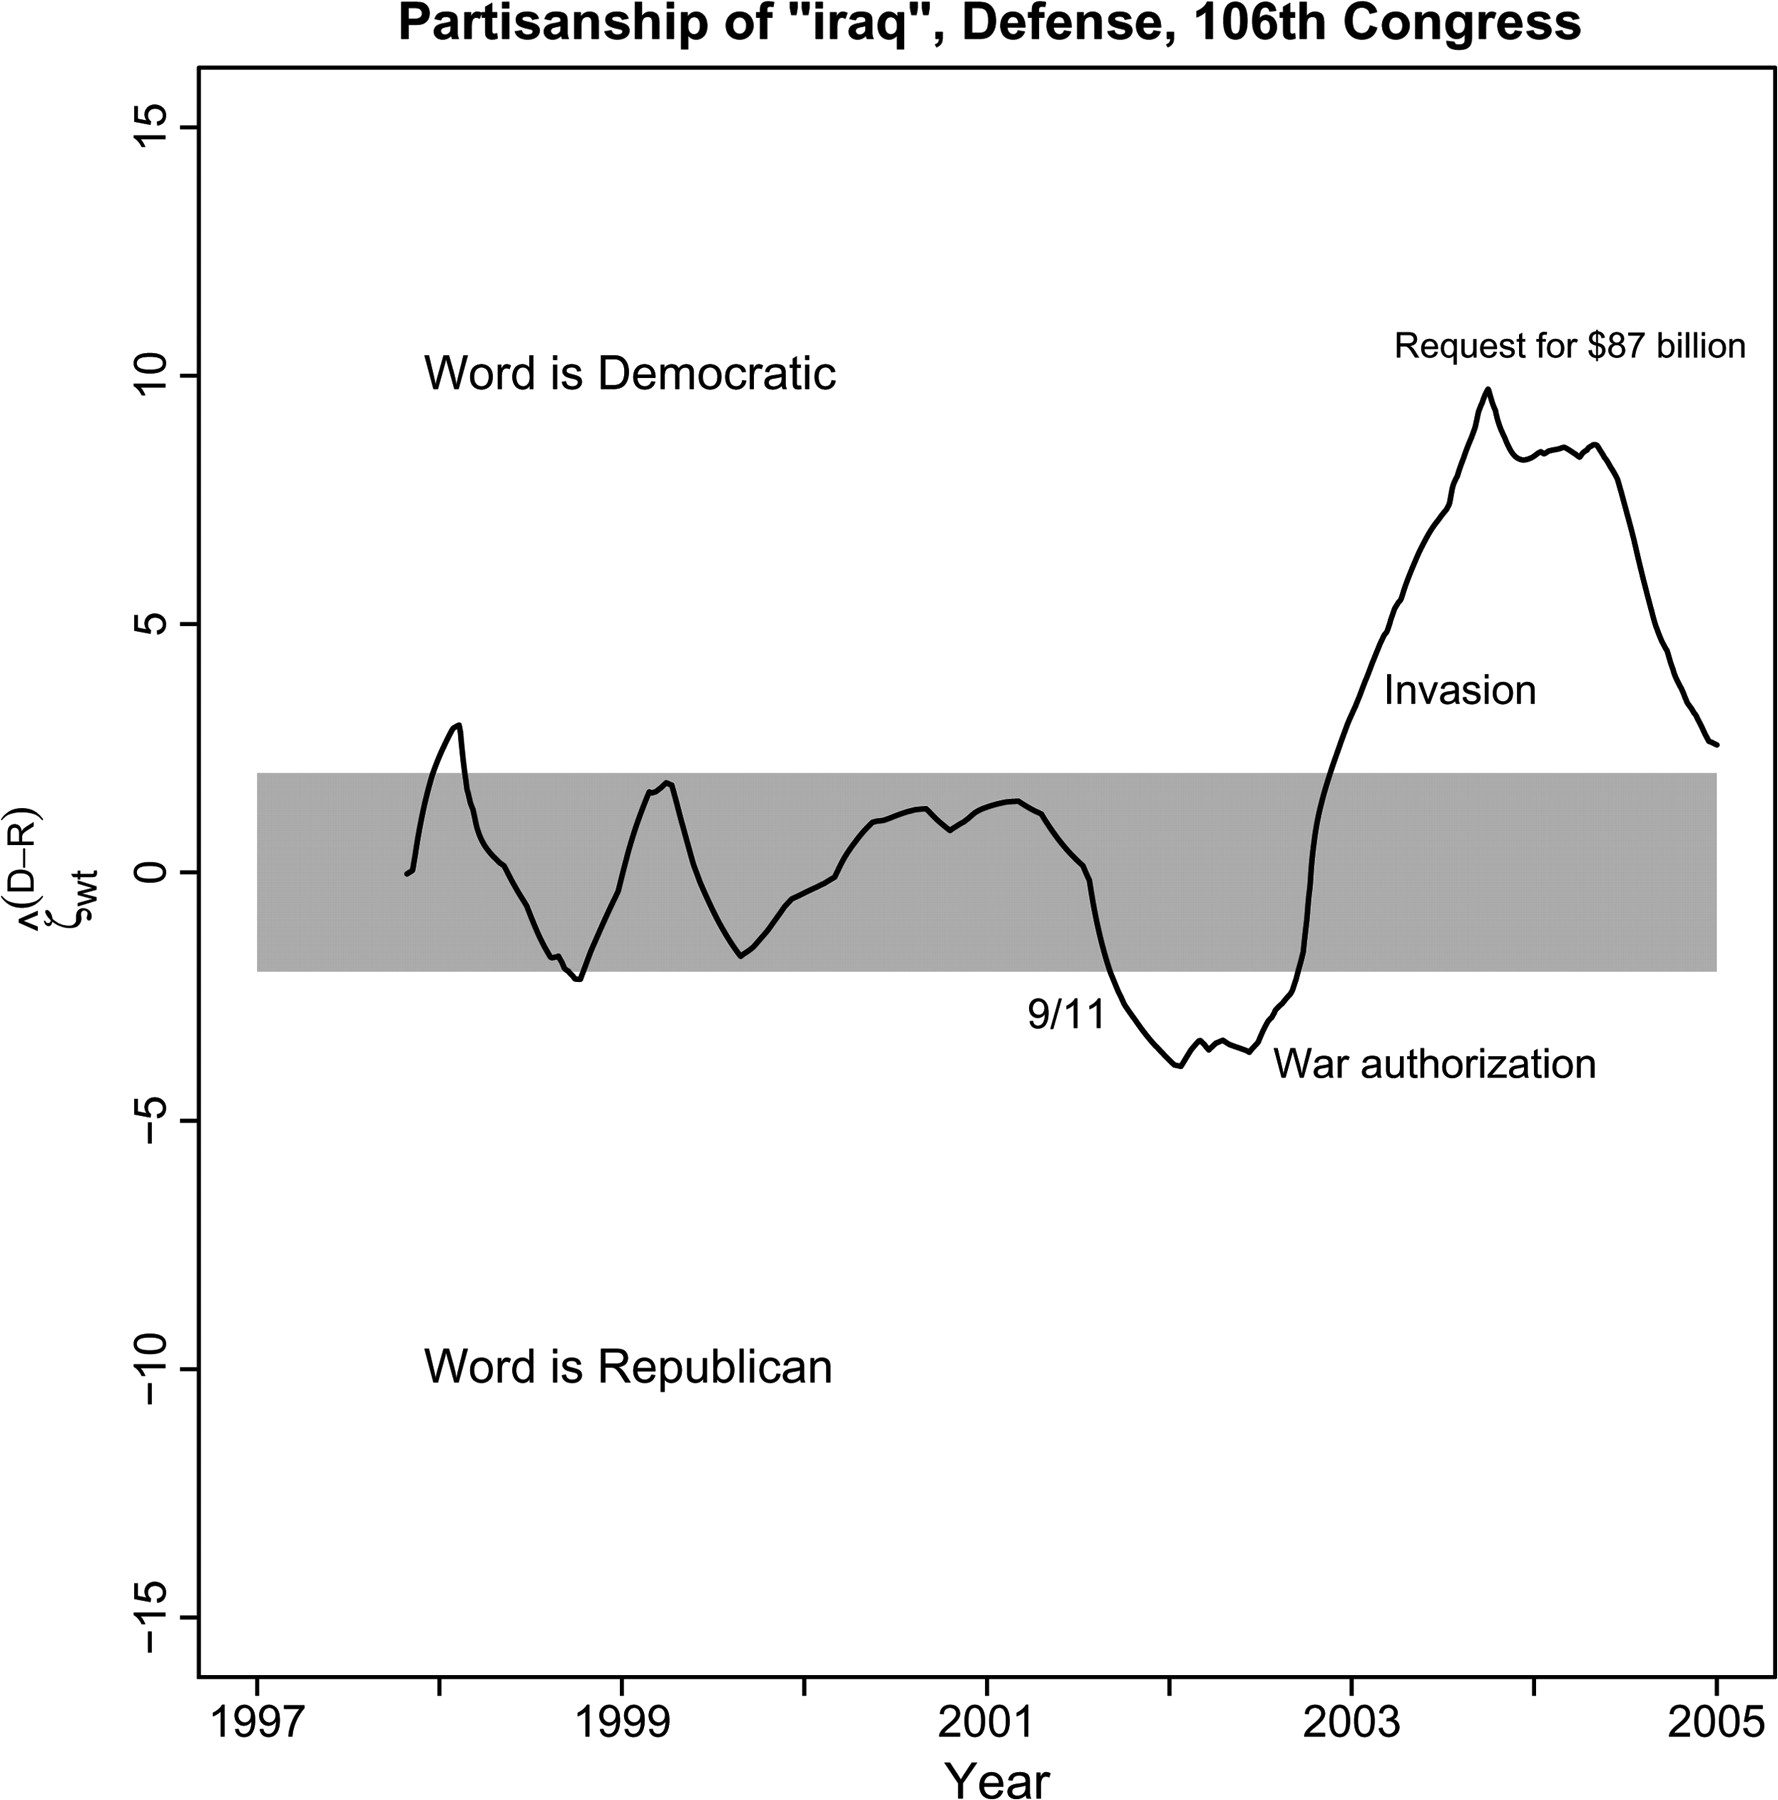
\includegraphics[scale=.21]{fightin2}}




%
%\slide{Classification when Categories\\are Unknown}
%
%
%\centerline{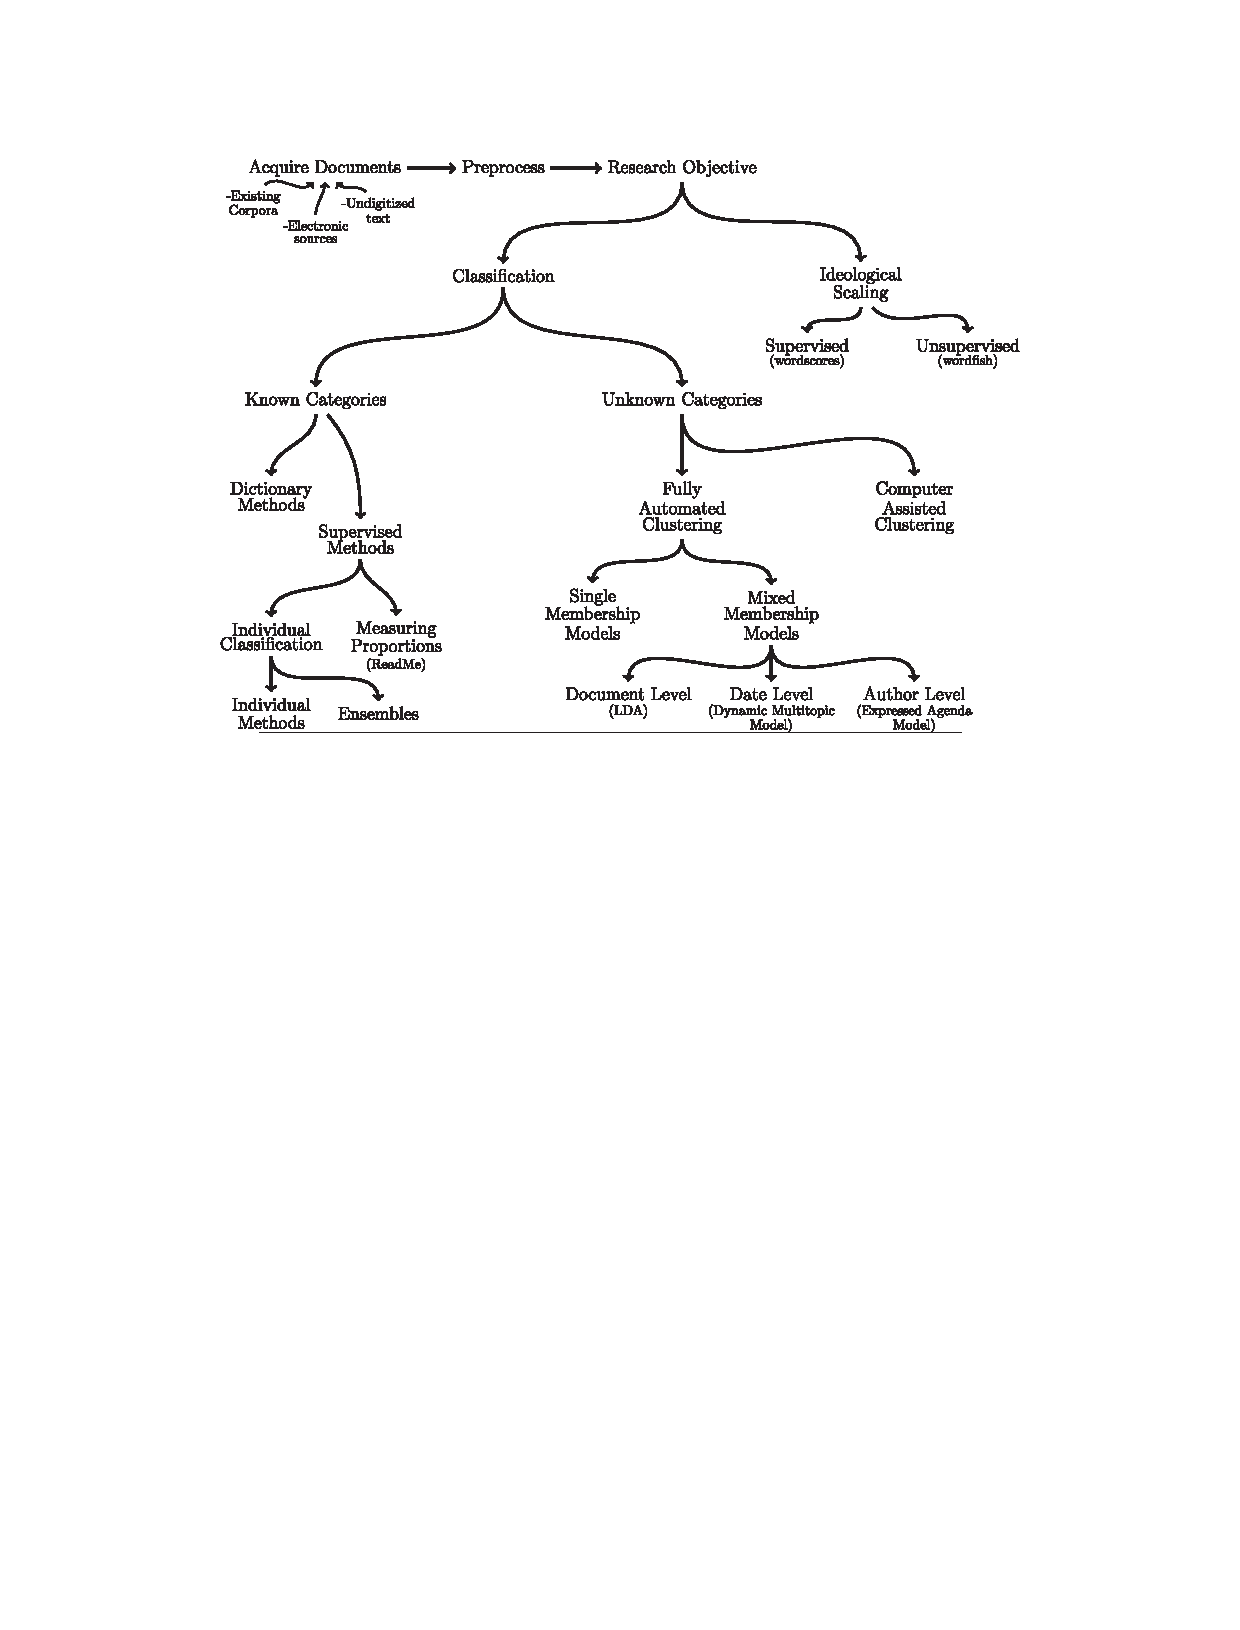
\includegraphics[scale=1.24]{grimmerovreview.pdf}}
%
%
%
%\slide{Topic Models}
%
%
%Supervised and dictionary methods assume well-defined set of categories. Perhaps you don't want to, or (more likely) can't, classify documents or write a dictionary yourself.
%
%
%Is it still possible to model the proportions of themes in text?  Yes!
%
%
%Topic models (Blei, Ng and Jordan, 2003; Blei and Lafferty, 2009) are full probability models that
%\ita
%\itm weaken the constraints required in dictionary based content analysis
%\itm may do what you want.  Or not\ldots
%\itz
%
%These are \textit{exploratory} methods that work best
%with \textit{large amounts} of text with a \textit{thematic} structure.
%
%
%\slide{Topic Models}
%
%Topic models represent documents as a mixture of topics.
%
%All documents in the text collection (e.g. Congressional bills) share the same set of topics, but each document (e.g. individual bill) exhibits a different proportion of topics.
%
%
%
%Documents are observed, the rest is not:
%\ita
%\itm topics
%\itm the per-document topic distribution
%\itm  the per-document per-word topic assignment.
%\itz
%%\centerline{\includegraphics[scale=.6]{topic-model2}}
%
%\slide{Topic Models: LDA}
%
%
%\centerline{\includegraphics[scale=.6]{topics}}
%
%
%\slide{Topic Models: LDA}
%
%\centerline{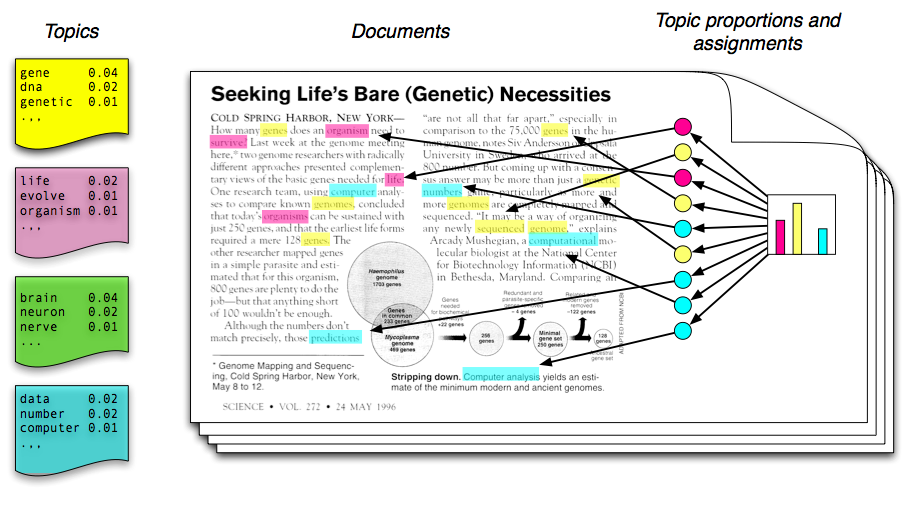
\includegraphics[scale=.6]{topics2}}
%
%
%\slide{Topic Models: LDA}
%
%Latent Dirichlet Allocation (LDA):
%
%Dirichlet distribution describes knowledge about a vector of probabilities, here the probabilities of topics per document.
%
%A generative model:
%
%For example, with two topics, you may choose that a document is 1/3 about topic A and 2/3 about topic B.
%
%
%\slide{Topic Models: LDA}
%
%\centerline{\includegraphics[scale=.6]{topic-model}}
%
%
%\slide{Topic Models: LDA}
%
%LDA reverses the generative process to find the hidden structure that is likely to have generated the observed documents (essentially using the co-occurrence of words across documents)
%
%
%Topic models add:
%\ita
%\itm A \textit{probabilistic} view of the relationship between W (observed word), Z (per-word topic assignment) and $\theta$ (per-document topic proportions)
%\itm Topics = distribution over a fixed vocabulary
%\itm Full statistical framework for learning most aspects of the relationship
%\itz
%
%\slide{Topic Models: LDA}
%
%But:
%\ita
%\itm topic models take away substantive control: you do not get to assert what the topics \textit{mean}
%\itm they return only one single clustering
%\itz
%
%%
%%\slide{Variations: Dynamic Topic Models}
%
%%\centerline{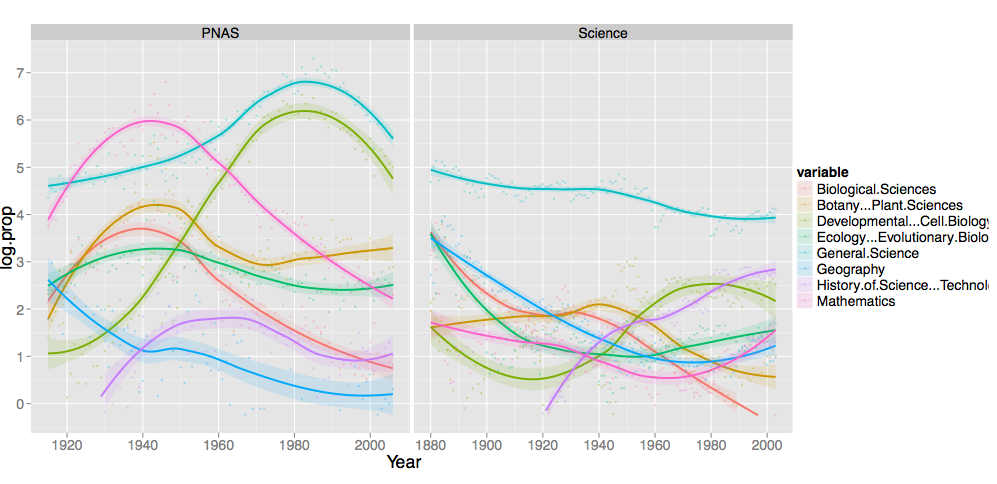
\includegraphics[scale=.7]{dynamics}}
%
%%\slide{Variations: Dynamic Topic Models}
%
%%Quinn et al. analyze 118,065 such congressional speeches from 1997-2004.
%
%%$\theta$ has Markovian dynamics for smooth movement in topic proportions.
%
%%Note: This does \textit{not} allow variation in the way topics are expressed in words
%%\ita
%%\itm Why not?
%%\itz
%
%
%%\slide{Applications: Policy Agenda}
%%
%%\centerline{\includegraphics[scale=.5]{911}}
%
%\slide{Interpreting Topics}
%
%\centerline{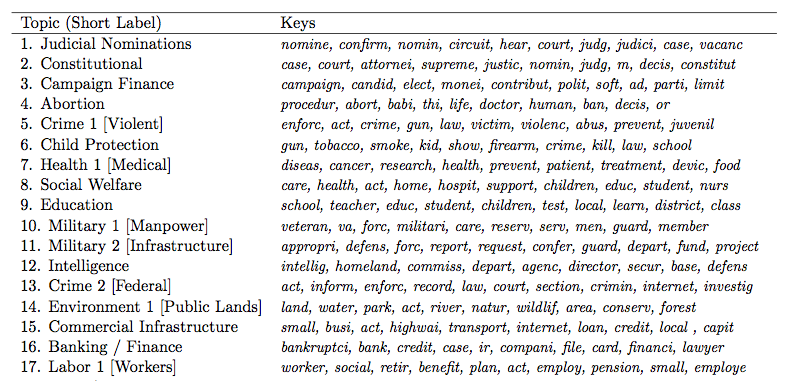
\includegraphics[scale=.8]{topic-words}}
%
%{\footnotesize (Quinn et al. 2010)}
%
%\newpage
%
%%\centerline{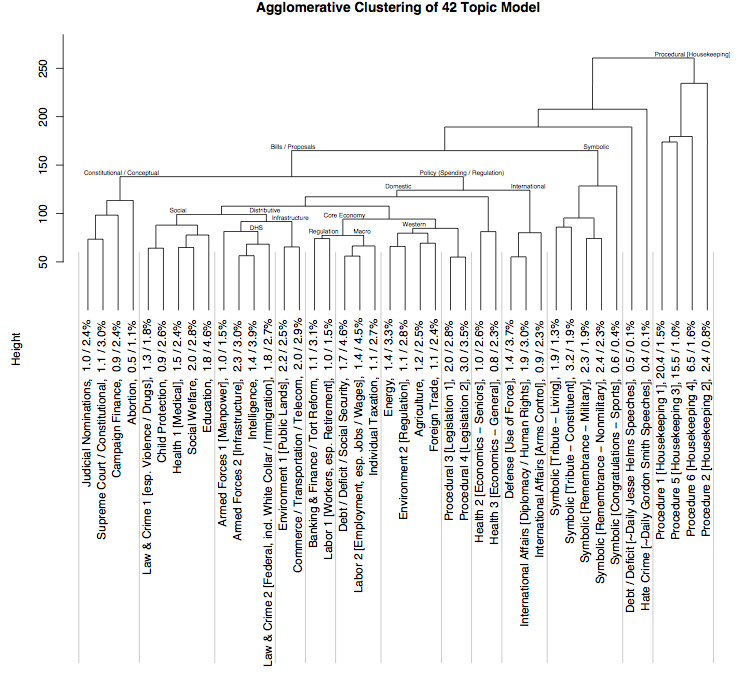
\includegraphics[scale=.58]{topic-clustering}}
%%
%%{\footnotesize (Quinn et al. 2010)}
%%%\newpage
%%
%%%\centerline{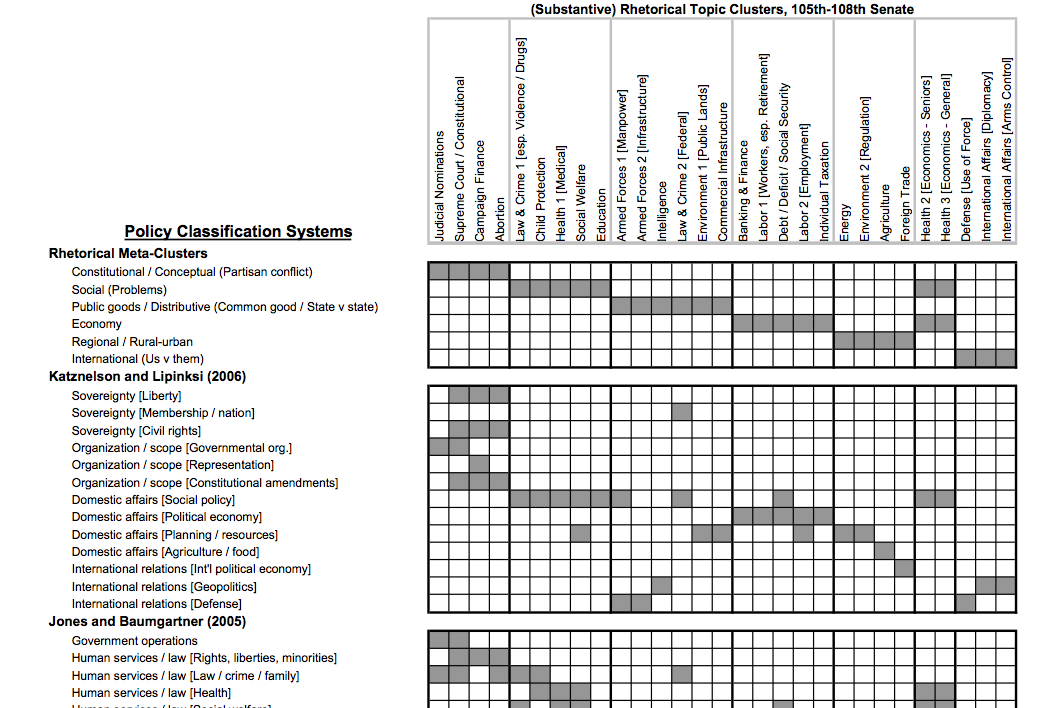
\includegraphics[scale=.7]{other-schemes}}
%%
%\slide{Variations: Expressed Agenda Model}
%
%In a simpler variation on LDA, Grimmer (2010) defines an expressed agenda model for Senate press releases. \vspace{5mm}
%~\\
%\centerline{\includegraphics[scale=2.2]{grimmer}}
%
% Here there are \textit{not} multiple topics per senatorial press release, but senators are at the mixed membership level (i.e. mix attention to topics).
%
%Goal: estimate the topics in the data (all Senate press releases), assign press releases to their likely topic, and measure attention  Senators dedicate to estimated topics.
%
%
%\slide{Topic Models: How many topics?}
%
%One of the most difficult questions in unsupervised learning.
%
%Grimmer (2010) applies a variation of a topic model on Senate press releases to measure expressed agendas.
%
%
%
%\begin{quote}
%The results presented in this paper [\ldots] assume there are 43 topics present in the data. I varied the number of assumed topics from only five topics, up to 85 different topics. Assuming too few topics resulted in distinct issues being lumped together, whereas too many topics results in several clusters referring to the same issues. \textbf{During my tests, 43 issues represented a decent middle ground.}
%(Grimmer 2010, p.12)
%\end{quote}
%
%
%\slide{Labeling topics}
%
%
%\begin{enumerate}
%
%\item Randomly select documents from each topic with a high posterior probability of belonging to that topic, then read and manually assign a label (compare cluster quality)
%
%\item Use the model output to identify words that distinguish the documents in a particular topic
%
%
%
%\item Validate with external events (predictive validity)
%
%\end{enumerate}
%
%\slide{Labeling Topics}
%
%
%
%\centerline{\includegraphics[scale=1.2]{grimmertopics}}
%
%\slide{Labeling Topics}
%
%
%\centerline{\includegraphics[scale=2]{grimmerimmig}}
%
%
%Senators issue press releases on the topic with the label "immigration" when important votes in the Senate take place.
%
%%\slide{Assessing Validity of Topics}
%%
%%
%%
%%Expectation: Members of Congress want to be perceived as being effective policy makers and emphasize issues that come before committees they lead (Fenno 1978).
%%
%%Grimmer compares committee leaders' average attention to an issue under the committee's jurisdiction with the average attention among the other Senators.
%%
%%\slide{Assessing Validity of Topics }
%%
%%\centerline{\includegraphics[scale=0.9]{grimmercomm}}
%%
%%Committee leaders pay more attention to their committee's issues.
%%
%\slide{Assessing Validity of Topics (Grimmer)}
%
%Expectation:  Senators who tout  appropriations secured for a state in their press releases view these appropriations essential to their electoral security and should be less likely to vote for earmark reform.\vspace{10mm}
%
%\centerline{\includegraphics[scale=1.5]{grimmerearmark}}
%
%%
%
%
%\slide{Questions}
%%
%%\slide{Doing This At Home}
%%
%%Most methods require \textit{some programming skill} to use
%%\ita
%%\itm Note the prevalence of multi-author papers in this area of political science\ldots
%%\itz
%%Tools:
%%\ita
%%\itm Classification: Mallet, LingPipe, WEKA for Java; NLTK for Python; R packages in the machine learning `View';
%%BMR/BLR.
%%\itm Topic Models: R packages topicmodels, lda; LDA-C and get yourself on the `topicmodels' mailing list
%%\itm Reading: Manning and Sch\"{u}tze 1999; Jurafsky and Martin 2000; Bishop 2006
%%\itz
%%
%
%
%%\slide{Biased Training Data}
%%
%%\slide{Readme}
%%
%%How to answer the question
%%
%%The sample is not informative about $P(\theta)$ (it's not balanced the right way)
%%
%%But it \textsl{is} informative about $P(W_1\ldots W_V \mid \theta)$
%%
%%Readme treats document classification like a \textsl{regression} problem
%%\begin{align*}
%%P(W_1\ldots W_V) & = P(W_1\ldots W_V \mid \theta)~ P(\theta)\\
%%Y                & = X \beta\\
%%\beta            & = (X^TX)^{-1} X^TY
%%\end{align*}
%%Actually, like a \textsl{calibration} problem\ldots
%%
%%\slide{Readme}
%%
%%Extremely high dimensional data matrices require special methods
%%
%%On the other hand, the SVM classifier took more than 8 days to run
%%
%%\slide{Readme vs SVM}
%%
%%\centerline{\includegraphics[scale=.85]{affect-blogs}}
%%
%%\slide{Why Readme might be useful for you}
%%
%%Sometimes the sample content proportions are \textsl{not} the population proportions, e.g.
%%\ita
%%\itm You have equal numbers of documents/words on the economy, defense, and animal welfare
%%\itz
%%Classifiers are constructing
%%\begin{align*}
%%P_{\text{sample}}(\theta \mid D) &~~\propto~~ P(D \mid \theta) ~\times~ P_{\text{sample}}(\theta)
%%\end{align*}
%%but $P_{\text{sample}}(\theta) ~\neq~ P(\theta)$, so the posterior is probably wrong too
%%If you \textsl{knew} the population proportions you'd use them, e.g. as case weights in the classifier
%%
%%\slide{Correcting for Sample Bias}
%%
%%One method of correction uses the classifier's confusion matrix (McLachlan and Basford, 1988)
%%
%%Use the sample data to estimate $M$, a matrix of classifier \textsl{mistakes}
%%\begin{align*}
%%M_{jk} &~~=~~ P(\hat{\theta}=k \mid \theta=j)
%%\end{align*}
%%
%%Intuition for two categories:
%%\begin{align*}
%%E[C_j] &~~=~~ P(\theta=j)\,M_{jj} ~\,+~ P(\theta=k)\,M_{kj}\\
%%E[C_k] &~~=~~ P(\theta=j)\,M_{jk} ~+~ P(\theta=k)\,M_{kk}
%%\end{align*}
%%So we can estimate the true proportion of units in each content category by solving this linear system for $P(\theta)$
%%
%%\slide{Correcting for Sample Bias}
%%
%%And that is what Readme does for document classification
%%

\end{frame}
\begin{frame}[t]\frametitle{Designing a Content Analysis:\\Issue to Consider}

\ita

\itm Validity: does measurement reflect the truth?
\itm Replicability: can you repeat the procedure?
\itm Uncertainty: how uncertain are estimates?
\itm Accuracy: proportion of correctly classified documents?
\itm Precision: proportion of documents assigned a category $i$ that are actually about this category?
\itm Recall: proportion of documents in category $i$ classified correctly?
\itm Dictionary: substantive, theory-driven, vocabulary from training set
\itz

\end{frame}
\begin{frame}[t]\frametitle{Validity and Reliability}

\begin{center}\includegraphics[scale=.15]{targets}\end{center}

\end{frame}
\begin{frame}[t]\frametitle{Validity and Reliability}

\begin{center}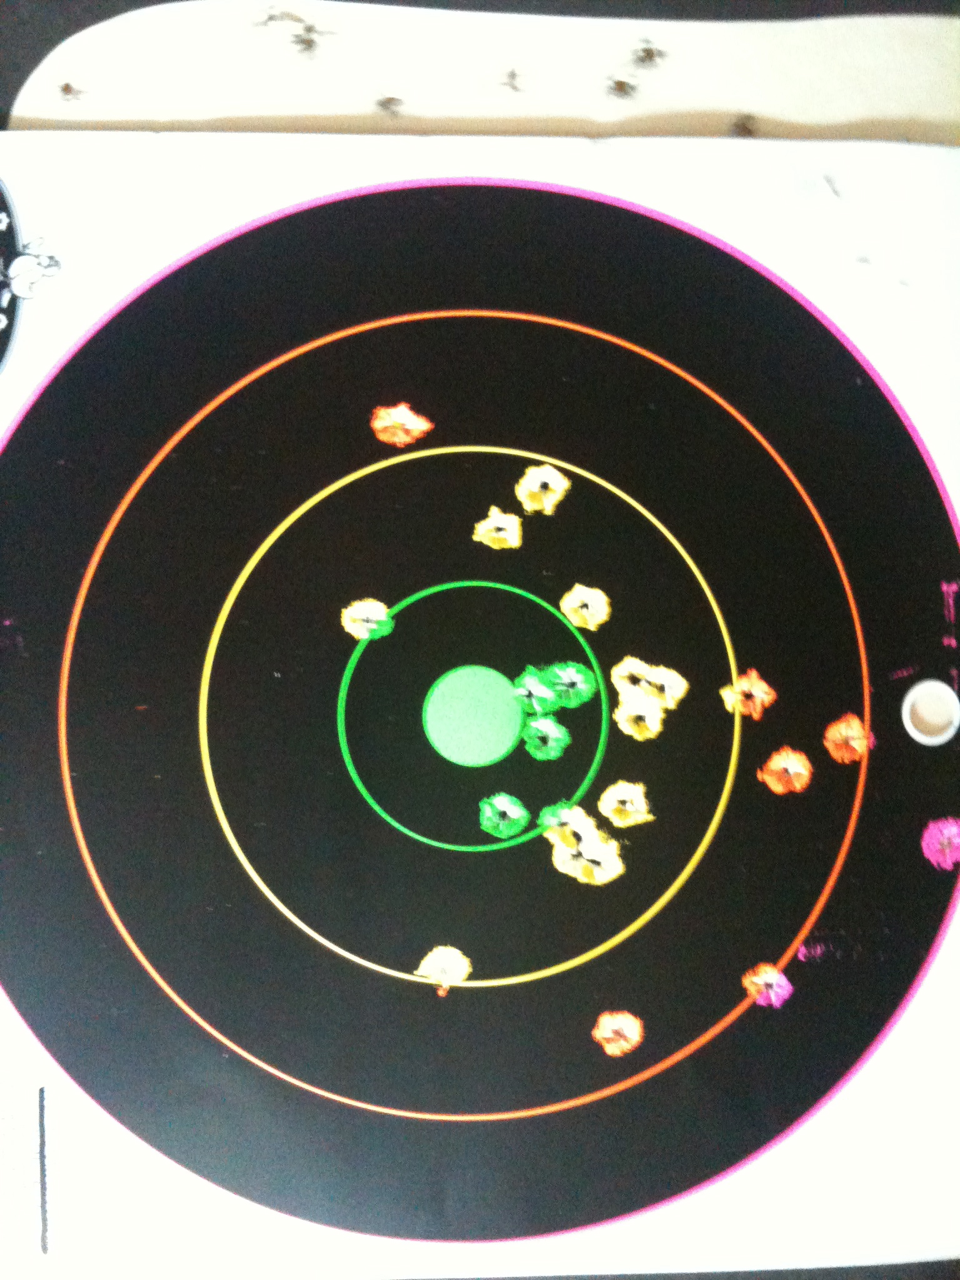
\includegraphics[scale=.2,angle=270]{wl-targets3}
~~~~~~~~~~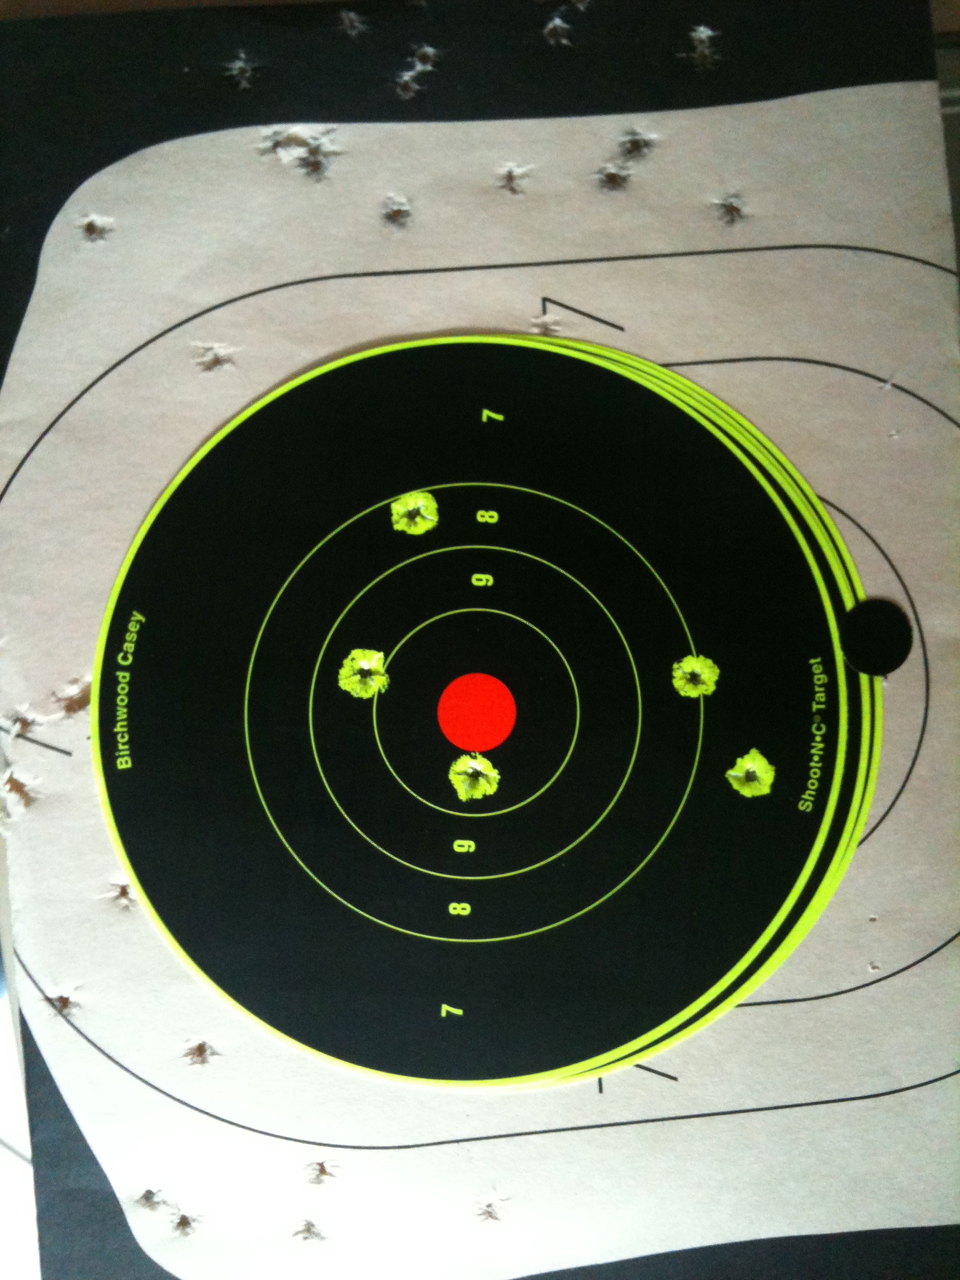
\includegraphics[scale=.2,angle=270]{wl-targets4}\end{center}




\end{frame}
\begin{frame}[t,fragile]\frametitle{Constructing Dictionaries}

Always a trade-off between {\it precision} and {\it recall}.

\ita
\itm \textbf{Precision}: proportion of words used the way your dictionary assumes
\itm \textbf{Recall}: proportion of words used that way that are in your dictionary
\itz

Depends on {\it a priori} knowledge on categories

\ita

\itm Unknown categories: topic model $\rightarrow$ look at words strongly associated with discovered topics

\itm Known categories: human coding of entire document, discover discriminatory words from classification analysis

\itm Keyword in context analyses allow you to scan all contexts of a word
\ita
\itm How many of them are the sense or usage you want?
\itz

\itz


%
%\slide{Solutions}
%
%\newpage
%
%\centerline{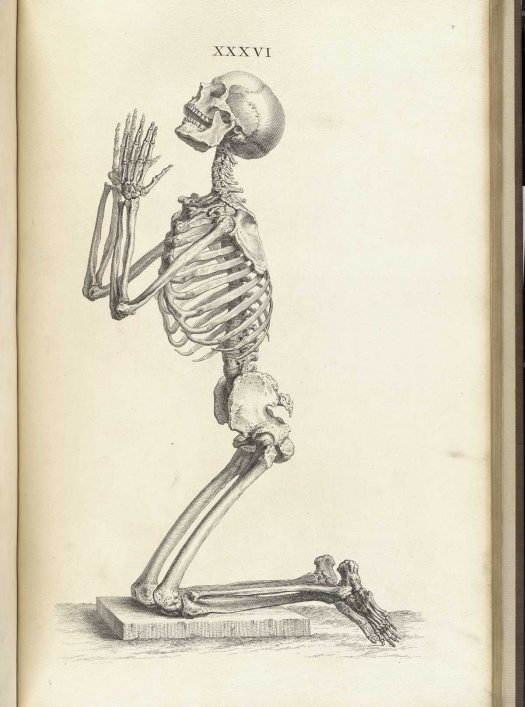
\includegraphics[scale=.7]{praying-skeleton}}
%
%\slide{Solutions: Try to Avoid Measurement Error}
%
%A non-intuitive fact about content dictionaries:
%\ita

%\itz
%\textit{always} trade-off\ldots
%
%\slide{Intuition: Precision and Recall}
%
%\centerline{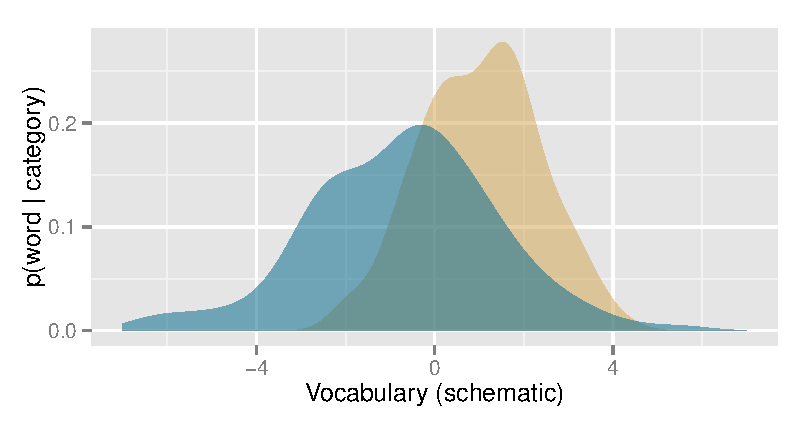
\includegraphics[scale=1.7]{schematic-vocab}}
%
%\slide{Solutions}
%
%
%
%
\end{frame}

\end{document}



\begin{frame}[t,fragile]\frametitle{Ideological Position and SVM}

Support Vector Machines are the state of the art for classification accuracy (just)
\ita
\itm Non-statistical (maximum margin) method
\itm Computationally demanding
\itm Non-intuitive parameterization
\itz

Question: What are the ideological positions of senators?

Yu et al. use the 25 most liberal and 25 most conservative senators (chosen via DNOMINATE scores) to train a SVM classifier to classify senators by their speeches:


%\slide{Ideological Position and SVM}

%\centerline{\includegraphics[scale=.9]{yu-5}}

\end{frame}
\begin{frame}[t,fragile]\frametitle{Ideological positions}

Up to 94\% correct classification on these 50 senators

Only up to 64\% correct classification trained and tested on moderate senators (the middle 50)

\end{frame}
\begin{frame}[t,fragile]\frametitle{A Theory of Moderates (1)}

\begin{quotation}
``[This is] a new way to think about
moderate senators which uncovers a hidden assumption in the spatial representation of
ideologies. According to the Poole-Rosenthal approach, the ideological position of
members of Congress is identical to their ideal point in a multi-dimensional.
But once we
fix an ideal point, moderate ideological positions are just as well-defined and precise as
``extreme'' positions.''
\end{quotation}

\end{frame}
\begin{frame}[t,fragile]\frametitle{A Theory of Moderates (2)}

\begin{quotation}
``There is, however, a different way to conceptualize moderates. We
are not aware of a formal representation of this idea, but it does appear from time to time
in popular political discourse. The idea here is that moderate liberals and conservatives
do not constitute a separate position, but are simply \textsl{more blurry} versions of their extreme
counter-parts.''
\end{quotation}

\end{frame}
\begin{frame}[t,fragile]\frametitle{A Theory of Moderates (3)}

Predictions:
\ita
\itm If moderates are `blurry' extremists then a classifier trained on moderate example would do less in classifying both moderates and extremists
\itm If moderate is a position, then a classifier trained on moderate example would do very well on moderates and not well on extremists
\itz

\end{frame}
\begin{frame}[t,fragile]\frametitle{A Theory of Moderates (4)}

\centerline{\includegraphics[scale=.9]{yu-5}}

\end{frame}
\begin{frame}[t,fragile]\frametitle{A Theory of Moderates}

\centerline{Do we believe this?}

\end{frame}

\plain{}



%:RESIDUAL MATERIAL

%%%%%%%%%%%%%%%%%%%%%%%
%% part 2 %%%%%%%%%%%%%
%%%%%%%%%%%%%%%%%%%%%%%



%%%%%% Measurement here



\begin{frame}[t,fragile]\frametitle{Measurement models}

Substantive assumption
\begin{quotation}
\noindent
Unobserved $\theta$ \textsl{causes} observations $W_1, W_2, W_3,\ldots, W_V$
\end{quotation}
Statistical assumption
\begin{quotation}
$P(W_1,\ldots, W_V \mid \theta) ~=~ \prod_w^{V} P(W_w \mid {\theta})$
\end{quotation}
Once $\theta$ is known, variation in $W_1, W_2, W_3,\ldots, W_V$
is random.

\end{frame}
\begin{frame}[t,fragile]\frametitle{Measurement models}

General Principle:
\ita
\itm Effects of a common cause will be correlated, until it is conditioned on, or controlled for
\itz

You've seen this before, e.g
\ita
\itm good regression models make observations random, conditional on the explanatory variables
\itz


\end{frame}
\begin{frame}[t,fragile]\frametitle{Measurement Models}

Measurement model:
\ita
\itm Fit a model of $W_1 \ldots W_V \Leftarrow \theta$\\
then \textit{reverse} it to get an estimate of $\theta$
\itz
Examples:
\ita
\itm Factor Analysis
\itm Latent Class analysis
\itm Item Response Theory
\itm Structural Equation Models
\itz

\end{frame}
\begin{frame}[t,fragile]\frametitle{Measurement Models}

Advantage: Requires no information about $Z$s or $\theta$s

Disadvantage: Leans heavily on functional and distributional assumptions

Let's look at some possible assumptions\ldots

\end{frame}
\begin{frame}[t,fragile]\frametitle{How might $\theta$ affect words?}

word prob. depends on \textit{identity} of $\theta$\\
(via a category label Z)

word prob. depends on the \textsl{magnitude} of $\theta$

word prob. depends on the \textsl{distance} of $\theta$ from a point



%%%%%%%%%%%%%% scaling %%%%%%%%%%%%%

\end{frame}
\begin{frame}[t,fragile]\frametitle{Of Left and Right}


Spatial politics assumptions:
\ita
\itm Policy preferences are \textit{positions} or \textit{ideal points} on policy \textit{dimensions}
\itm There exists a \textit{low-dimensional space} that explains the multitude of positioning information available in observations of politics
\itz
Take everyday talk about 'left' and 'right' seriously.

Political representation is effective -- democratic, legitimate -- if politicians' preferences have the \textsl{right relationship} to citizens' preferences.

\end{frame}
\begin{frame}[t,fragile]\frametitle{Raw Materials of Left and Right}

Quantitative positioning information:
\ita
\itm Votes in a legislature (obvious, but biased)
\itm Answers to survey questions (unbiased but only sometimes possible)
\itm Structured qualitative analysis of manifestos (e.g. Pellican, Krouwel)
\itm Counts of policy promises or assertions in a manifesto or speech (Budget et al.)

\itm Frequencies of individual words
\itz

\end{frame}
\begin{frame}[t,fragile]\frametitle{Of Left and Right}

\begin{center}
\includegraphics[scale=.3]{local-maastricht}
\end{center}


Keiskompass (see also Wahl-o-mat).


\end{frame}
\begin{frame}[t,fragile]\frametitle{Senate Speeches (Monroe et al.)}

\begin{center}
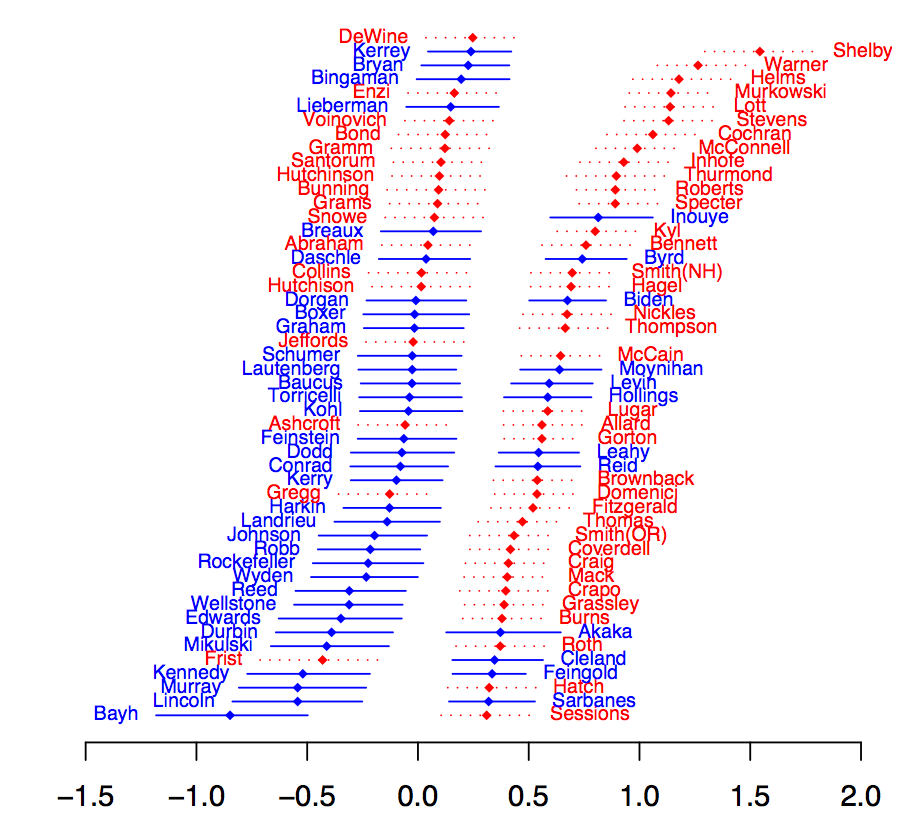
\includegraphics[scale=.2]{senator-ip-monroe-maeda}
\end{center}

\end{frame}
\begin{frame}[t,fragile]\frametitle{UK and IE Parties on the Economy}

\begin{center}
\includegraphics[scale=.25]{wordscores-uk-ie}
\end{center}


\end{frame}
\begin{frame}[t,fragile]\frametitle{2009 IE Budget Debate}

\begin{center}
\includegraphics[scale=.6]{clean-snap}
\end{center}

\end{frame}
\begin{frame}[t,fragile]\frametitle{Scaling Model (Proksch and Slapin)}

Assumptions about $P(W_1\ldots W_V \mid \theta)$
\begin{align*}
\log  \lambda_{ij} &~=~ \psi_j ~+~ \beta_j\theta_i ~+~  \alpha_i
\end{align*}

$\theta_i$ is the expressed position of a text

\end{frame}
\begin{frame}[t,fragile]\frametitle{Scaling Model (Proksch and Slapin)}

Assumptions about $P(W_1\ldots W_V \mid \theta)$
\begin{align*}
\log  \lambda_{ij}  &~=~ \psi_j ~+~ \beta_j\theta_i ~+~  \alpha_i
\end{align*}

$\alpha_i$ is a constant term controlling for document length

\end{frame}
\begin{frame}[t,fragile]\frametitle{Scaling Model (Proksch and Slapin)}

Assumptions about $P(W_1\ldots W_V \mid \theta)$
\begin{align*}
\log  \lambda_{ij}  &~=~ \psi_j ~+~ \beta_j\theta_i ~+~  \alpha_i
\end{align*}

The \textsl{sign} of $\beta_j$ represents the \textsl{ideological direction} of $W_j$

\end{frame}
\begin{frame}[t,fragile]\frametitle{Scaling Model (Proksch and Slapin)}

Assumptions about $P(W_1\ldots W_V \mid \theta)$
\begin{align*}
\log  \lambda_{ij}  &~=~ \psi_j ~+~ \beta_j\theta_i ~+~  \alpha_i
\end{align*}

The \textsl{magnitude} of $\beta_j$ represents the \textsl{sensitivity} of the word to ideological differences among speakers or parties

\end{frame}
\begin{frame}[t,fragile]\frametitle{Scaling Model (Proksch and Slapin)}

Assumptions about $P(W_1\ldots W_V \mid \theta)$
\begin{align*}
\log  \lambda_{ij}  &~=~ \psi_j ~+~ \beta_j\theta_i ~+~  \alpha_i
\end{align*}

$\psi_j$ is a constant term for the word (larger for high frequency words).


\end{frame}
\begin{frame}[t,fragile]\frametitle{Scaling Model (Proksch and Slapin)}
\begin{center}
\includegraphics[scale=.3]{log-lambda.pdf}\hfill
\includegraphics[scale=.3]{lambda.pdf}
\end{center}

The underlying Poisson regression model reflects a \textit{multiplicative} relationship between position and words used

\end{frame}
\begin{frame}[t,fragile]\frametitle{Marginal Effects}

British National Party manifesto for 2009 EU elections

\end{frame}
\begin{frame}[t,fragile]\frametitle{Marginal Effects}

\footnotesize
Immigration is out of control.
\normalsize

\end{frame}
\begin{frame}[t,fragile]\frametitle{Marginal Effects}

\footnotesize
Immigration is out of control.
\textbf{Britain's population is now over 60 million and rising, solely due to immigration.}
\normalsize

\end{frame}
\begin{frame}[t,fragile]\frametitle{Marginal Effects}

\footnotesize
Immigration is out of control.
Britain's population is now over 60 million and rising, solely due to immigration.
\textbf{Not only is Britain increasingly overcrowded but the fact is that a country is the product of its people  and
if you change the people you will inevitably change the nature of the country.}
\normalsize

\end{frame}
\begin{frame}[t,fragile]\frametitle{Marginal Effects}

\footnotesize
Immigration is out of control.
Britain's population is now over 60 million and rising, solely due to immigration.
Not only is Britain increasingly overcrowded but the fact is that a country is the product of its people  and
if you change the people you will inevitably change the nature of the country.
\textbf{We want Britain to remain - or return to - the way it has traditionally been.}
\normalsize

\end{frame}
\begin{frame}[t,fragile]\frametitle{Marginal Effects}

\footnotesize
Immigration is out of control.
Britain's population is now over 60 million and rising, solely due to immigration.
Not only is Britain increasingly overcrowded but the fact is that a country is the product of its people  and
if you change the people you will inevitably change the nature of the country.
We want Britain to remain - or return to - the way it has traditionally been.
\textbf{We accept that Britain will always have ethnic minorities and
have no problem with this as long as they remain minorities and
neither change nor seek to change the fundamental culture and identity of the indigenous peoples of the British Isles.}
\normalsize

\end{frame}
\begin{frame}[t,fragile]\frametitle{Marginal Effects}

\footnotesize
\ldots fundamental culture and identity of the indigenous peoples of the British Isles.
\textbf{The current open-door policy and unrestricted uncontrolled immigration is leading to higher crime rates, demand for more housing (driving prices out of the reach of young people), severe strain on the environment, traffic congestion, longer hospital waiting list, lower educational standards, higher income taxes, lower wages, higher unemployment, loss of British identity, a breakdown in community spirit, more restrictive policing, higher council tax rates, a shortage of council homes, higher levels of stress and unhappiness and a more atomized society.}
\normalsize

\end{frame}
\begin{frame}[t,fragile]\frametitle{Marginal Effects}

~\\
Are we getting the point yet?

%\itm {sentence counts} (Budge 1994; Elff 2008)

\slide{}

\begin{center}
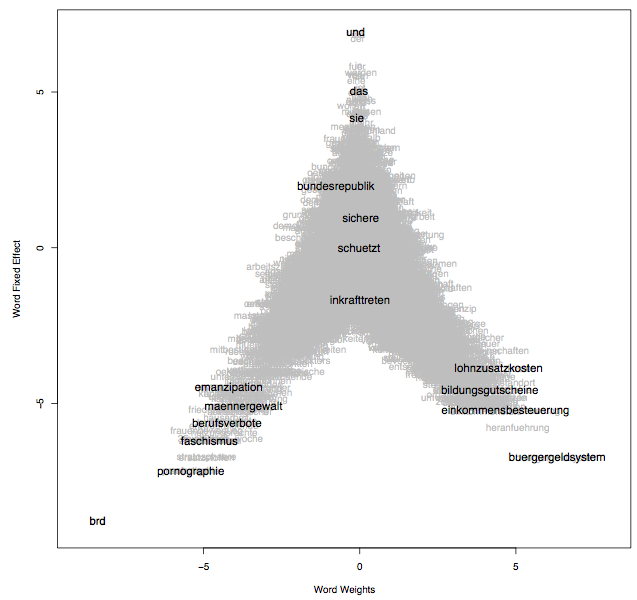
\includegraphics[scale=.35]{sp-informativeness.png}
\end{center}

\end{frame}
\begin{frame}[t,fragile]\frametitle{Whew!}

~\\
For the slower version, attend the ECPR Ljubljana Summer School in Methods and Techniques

Questions? Feuer frei!



\end{frame}
\begin{frame}[t,fragile]\frametitle{Good Old Logit}

It is tempting to go with methods we know (disciminative style)
\begin{eqnarray*}
\hat{\theta}_k &=& P(Z=k \mid W_1 \ldots W_V)\\
&=& \text{logit}^{-1}(\alpha + \beta_1 W_1 + \beta_2 W_2 + \ldots)
\end{eqnarray*}

This is a bad idea
\ita
\itm Why?
\itz

\end{frame}
\begin{frame}[t,fragile]\frametitle{Bad Old Logit}

The number of word types V is almost much larger than the number of documents D
\ita
\itm Many more `cases' than `variables'
\itm \textit{and} no constraint on possible solutions
\itz

Options (choose at least one):
\ita
\itm Move to a generative method based on $\theta \longrightarrow$ W
\itm Add constraints on the mapping between W and Z
\itz


\end{frame}
\begin{frame}[t,fragile]\frametitle{Evaluation: Accuracy, Precision and Recall}

We evaluate using estimates of
\begin{align*}
\text{P}(\hat{Z}=\text{`petitioner'} \mid Z=\text{`petitioner'}) && \text{Recall}  \\
\text{P}(Z=\text{`petitioner'} \mid \hat{Z}=\text{`petitioner'}) && \text{Precision}
\end{align*}
and
\begin{align*}
\text{P}(\hat{Z}=\text{`respondent'} \mid Z=\text{`respondent'}) && \text{Recall}  \\
\text{P}(Z=\text{`respondent'} \mid \hat{Z}=\text{`respondent'}) && \text{Precision}
\end{align*}

where $\hat{Z}$ is assigned by \textit{thresholding} $\theta$
\end{frame}



\end{document}
